\documentclass[]{book}
\usepackage{lmodern}
\usepackage{amssymb,amsmath}
\usepackage{ifxetex,ifluatex}
\usepackage{fixltx2e} % provides \textsubscript
\ifnum 0\ifxetex 1\fi\ifluatex 1\fi=0 % if pdftex
  \usepackage[T1]{fontenc}
  \usepackage[utf8]{inputenc}
\else % if luatex or xelatex
  \ifxetex
    \usepackage{mathspec}
  \else
    \usepackage{fontspec}
  \fi
  \defaultfontfeatures{Ligatures=TeX,Scale=MatchLowercase}
\fi
% use upquote if available, for straight quotes in verbatim environments
\IfFileExists{upquote.sty}{\usepackage{upquote}}{}
% use microtype if available
\IfFileExists{microtype.sty}{%
\usepackage{microtype}
\UseMicrotypeSet[protrusion]{basicmath} % disable protrusion for tt fonts
}{}
\usepackage{hyperref}
\hypersetup{unicode=true,
            pdftitle={Seminário Latinoamericano: Instrumentos y metodologias para un observatório de Clima y su impacto en la salud humana},
            pdfauthor={Sergio Ibarra-Espinosa, Universidade de São Paulo, sergio.ibarra@usp.br, ibarraespinosa.github.io},
            pdfborder={0 0 0},
            breaklinks=true}
\urlstyle{same}  % don't use monospace font for urls
\usepackage{natbib}
\bibliographystyle{apalike}
\usepackage{color}
\usepackage{fancyvrb}
\newcommand{\VerbBar}{|}
\newcommand{\VERB}{\Verb[commandchars=\\\{\}]}
\DefineVerbatimEnvironment{Highlighting}{Verbatim}{commandchars=\\\{\}}
% Add ',fontsize=\small' for more characters per line
\usepackage{framed}
\definecolor{shadecolor}{RGB}{248,248,248}
\newenvironment{Shaded}{\begin{snugshade}}{\end{snugshade}}
\newcommand{\AlertTok}[1]{\textcolor[rgb]{0.94,0.16,0.16}{#1}}
\newcommand{\AnnotationTok}[1]{\textcolor[rgb]{0.56,0.35,0.01}{\textbf{\textit{#1}}}}
\newcommand{\AttributeTok}[1]{\textcolor[rgb]{0.77,0.63,0.00}{#1}}
\newcommand{\BaseNTok}[1]{\textcolor[rgb]{0.00,0.00,0.81}{#1}}
\newcommand{\BuiltInTok}[1]{#1}
\newcommand{\CharTok}[1]{\textcolor[rgb]{0.31,0.60,0.02}{#1}}
\newcommand{\CommentTok}[1]{\textcolor[rgb]{0.56,0.35,0.01}{\textit{#1}}}
\newcommand{\CommentVarTok}[1]{\textcolor[rgb]{0.56,0.35,0.01}{\textbf{\textit{#1}}}}
\newcommand{\ConstantTok}[1]{\textcolor[rgb]{0.00,0.00,0.00}{#1}}
\newcommand{\ControlFlowTok}[1]{\textcolor[rgb]{0.13,0.29,0.53}{\textbf{#1}}}
\newcommand{\DataTypeTok}[1]{\textcolor[rgb]{0.13,0.29,0.53}{#1}}
\newcommand{\DecValTok}[1]{\textcolor[rgb]{0.00,0.00,0.81}{#1}}
\newcommand{\DocumentationTok}[1]{\textcolor[rgb]{0.56,0.35,0.01}{\textbf{\textit{#1}}}}
\newcommand{\ErrorTok}[1]{\textcolor[rgb]{0.64,0.00,0.00}{\textbf{#1}}}
\newcommand{\ExtensionTok}[1]{#1}
\newcommand{\FloatTok}[1]{\textcolor[rgb]{0.00,0.00,0.81}{#1}}
\newcommand{\FunctionTok}[1]{\textcolor[rgb]{0.00,0.00,0.00}{#1}}
\newcommand{\ImportTok}[1]{#1}
\newcommand{\InformationTok}[1]{\textcolor[rgb]{0.56,0.35,0.01}{\textbf{\textit{#1}}}}
\newcommand{\KeywordTok}[1]{\textcolor[rgb]{0.13,0.29,0.53}{\textbf{#1}}}
\newcommand{\NormalTok}[1]{#1}
\newcommand{\OperatorTok}[1]{\textcolor[rgb]{0.81,0.36,0.00}{\textbf{#1}}}
\newcommand{\OtherTok}[1]{\textcolor[rgb]{0.56,0.35,0.01}{#1}}
\newcommand{\PreprocessorTok}[1]{\textcolor[rgb]{0.56,0.35,0.01}{\textit{#1}}}
\newcommand{\RegionMarkerTok}[1]{#1}
\newcommand{\SpecialCharTok}[1]{\textcolor[rgb]{0.00,0.00,0.00}{#1}}
\newcommand{\SpecialStringTok}[1]{\textcolor[rgb]{0.31,0.60,0.02}{#1}}
\newcommand{\StringTok}[1]{\textcolor[rgb]{0.31,0.60,0.02}{#1}}
\newcommand{\VariableTok}[1]{\textcolor[rgb]{0.00,0.00,0.00}{#1}}
\newcommand{\VerbatimStringTok}[1]{\textcolor[rgb]{0.31,0.60,0.02}{#1}}
\newcommand{\WarningTok}[1]{\textcolor[rgb]{0.56,0.35,0.01}{\textbf{\textit{#1}}}}
\usepackage{longtable,booktabs}
\usepackage{graphicx,grffile}
\makeatletter
\def\maxwidth{\ifdim\Gin@nat@width>\linewidth\linewidth\else\Gin@nat@width\fi}
\def\maxheight{\ifdim\Gin@nat@height>\textheight\textheight\else\Gin@nat@height\fi}
\makeatother
% Scale images if necessary, so that they will not overflow the page
% margins by default, and it is still possible to overwrite the defaults
% using explicit options in \includegraphics[width, height, ...]{}
\setkeys{Gin}{width=\maxwidth,height=\maxheight,keepaspectratio}
\IfFileExists{parskip.sty}{%
\usepackage{parskip}
}{% else
\setlength{\parindent}{0pt}
\setlength{\parskip}{6pt plus 2pt minus 1pt}
}
\setlength{\emergencystretch}{3em}  % prevent overfull lines
\providecommand{\tightlist}{%
  \setlength{\itemsep}{0pt}\setlength{\parskip}{0pt}}
\setcounter{secnumdepth}{5}
% Redefines (sub)paragraphs to behave more like sections
\ifx\paragraph\undefined\else
\let\oldparagraph\paragraph
\renewcommand{\paragraph}[1]{\oldparagraph{#1}\mbox{}}
\fi
\ifx\subparagraph\undefined\else
\let\oldsubparagraph\subparagraph
\renewcommand{\subparagraph}[1]{\oldsubparagraph{#1}\mbox{}}
\fi

%%% Use protect on footnotes to avoid problems with footnotes in titles
\let\rmarkdownfootnote\footnote%
\def\footnote{\protect\rmarkdownfootnote}

%%% Change title format to be more compact
\usepackage{titling}

% Create subtitle command for use in maketitle
\providecommand{\subtitle}[1]{
  \posttitle{
    \begin{center}\large#1\end{center}
    }
}

\setlength{\droptitle}{-2em}

  \title{Seminário Latinoamericano: Instrumentos y metodologias para un observatório de Clima y su impacto en la salud humana}
    \pretitle{\vspace{\droptitle}\centering\huge}
  \posttitle{\par}
    \author{Sergio Ibarra-Espinosa, Universidade de São Paulo, \href{mailto:sergio.ibarra@usp.br}{\nolinkurl{sergio.ibarra@usp.br}}, ibarraespinosa.github.io}
    \preauthor{\centering\large\emph}
  \postauthor{\par}
      \predate{\centering\large\emph}
  \postdate{\par}
    \date{2019-09-10}

\usepackage{booktabs}
\usepackage{amsthm}
\makeatletter
\def\thm@space@setup{%
  \thm@preskip=8pt plus 2pt minus 4pt
  \thm@postskip=\thm@preskip
}
\makeatother

\begin{document}
\maketitle

{
\setcounter{tocdepth}{1}
\tableofcontents
}
\hypertarget{curso-de-r-contaminacion-atmosferica-y-mas}{%
\chapter*{Curso de R, contaminacion atmosferica y mas}\label{curso-de-r-contaminacion-atmosferica-y-mas}}
\addcontentsline{toc}{chapter}{Curso de R, contaminacion atmosferica y mas}

Este curso online contendra las sisgueinetes informaciones

\begin{itemize}
\tightlist
\item
  Sistemas de informacion con dartos de salud en Chile (gracias Paty Matus)
\item
  Impacto de las emisiones antropogenicas en la salud y clima
\item
  R desde Excel
\item
  Leer y procesar vectores espaciales con \textbf{sf} \citep{sf}
\item
  Leer y procesar informacion en grillas espaciales (raster) con stars\citep{stars} y raster\citep{raster}
\end{itemize}

\hypertarget{aprender-git}{%
\section*{Aprender Git}\label{aprender-git}}
\addcontentsline{toc}{section}{Aprender Git}

Para aprender GIT puedes ver:

\begin{itemize}
\tightlist
\item
  \url{https://git-scm.com/book/es/v1/Empezando}
\item
  \url{https://learngitbranching.js.org/}
\item
  \url{https://try.github.io/}
\end{itemize}

\hypertarget{clonar-este-contenido}{%
\section*{Clonar este contenido}\label{clonar-este-contenido}}
\addcontentsline{toc}{section}{Clonar este contenido}

Para clonar este contenido haz:

\begin{Shaded}
\begin{Highlighting}[]
\FunctionTok{git}\NormalTok{ clone https://github.com/ibarraespinosa/UBA.git}
\end{Highlighting}
\end{Shaded}

\hypertarget{intro}{%
\chapter{Sistemas de informacion con datos de salud en Chile}\label{intro}}

\begin{itemize}
\tightlist
\item
  Sistema de información en salud existentes
\item
  Enfasis en las fuentes de información y las escala temporal/espacial que manejan
\item
  Series de tiempo disponible por fuente
\item
  Instituciones a cargo de la captura, procesamiento y análisis
\item
  Disponibilidad de los datos e indicadores que producen
\item
  Otros
\end{itemize}

\hypertarget{encuesta-nacional-de-salud-ens}{%
\section{\texorpdfstring{\href{http://www.encuestas.uc.cl/ens/index.html}{Encuesta Nacional de Salud (ENS)}}{Encuesta Nacional de Salud (ENS)}}\label{encuesta-nacional-de-salud-ens}}

La ENS es una encuesta realizada por el Ministerio de Salud para identificar cuales son las
enfermedades que sufren y los tratamientos que reciben todas las personas con mas de 15 años
que viven en Chile. De esta forma es posible es posible realizar diagnosticos,
identificar problemas y formular politicas planes y proyectos para mejor la salud de las personas.

\begin{itemize}
\tightlist
\item
  \emph{Organismo responsable}: Ministerio de Salud, Departamento de Epidemiología\\
  Gobierno de Chile.\\
\item
  \emph{Organismo ejecutor}: Pontificia Universidad Católica de Chile (PUC).\\
\item
  \emph{Población objetivo}: Personas de 15 años y más, chilenas o extranjeras que residen habitualmente en viviendas particulares ocupadas, localizadas en zonas urbanas y rurales de las quince regiones de Chile.\\
\item
  \emph{Representatividad}: Nacional, regional y Urbano/Rural.\\
\item
  \emph{Modo de aplicación}: Entrevista personal en hogar (Sistema de captura electrónica: Tablet), aplicada por encuestador y profesional enfermera de acuerdo al tipo de cuestionario.\\
\item
  \emph{Período de trabajo de campo}: Agosto 2016 a marzo 2017\\
\item
  \emph{Tamaño muestral}: 6.233 encuestados, de los cuales 5.520 cuentan con exámenes de laboratorio de acuerdo a protocolo. 37,1\% hombres, 62,9\% mujeres.\\
\item
  \emph{Error muestral}: Error absoluto de muestreo de 2,6\% a nivel nacional, raíz del efecto de diseño de 1,797, estimaciones con 95\% de confianza y error relativo inferior a 30\%.
\end{itemize}

Algunos resultados:

\begin{itemize}
\tightlist
\item
  Consumo de tabaco: 66,7\% no fuma, 33,\$ fuma.
\item
  Consumo riesgoso de alcohol 11,7\%, 20,5\% hombres, 3,3\% mujeres.
\item
  Sedentarismo: 86,7\%, 83,3\% hombre, 90.0\% mujeres.
\item
  Estado nutricional: 1,3\% enfraquecido, 24,5\% normal, 39,8\% sobrepeso, 31,2\% obeso, 3,2\% obeso morbido.
\item
  Sospecha de hipertension: 27,6\%.
\item
  Sospecha de diabetes: 12,3\%.
\item
  Autoreporte de infarto agudo al miocardio: 3,3\%.
\item
  Autoreporte de ataque cerebro vascular: 2,6\%.
\end{itemize}

Fuentes:

\begin{itemize}
\tightlist
\item
  \url{https://www.minsal.cl/wp-content/uploads/2017/11/ENS-2016-17_PRIMEROS-RESULTADOS.pdf}
\item
  \url{https://www.minsal.cl/wp-content/uploads/2018/01/2-Resultados-ENS_MINSAL_31_01_2018.pdf}
\item
  \url{http://www.encuestas.uc.cl/ens/index.html}
\end{itemize}

\hypertarget{departamento-de-estadisticas-e-informaciones-de-salud}{%
\section{\texorpdfstring{\href{http://www.deis.cl/}{Departamento de Estadisticas e Informaciones de Salud}}{Departamento de Estadisticas e Informaciones de Salud}}\label{departamento-de-estadisticas-e-informaciones-de-salud}}

\begin{itemize}
\tightlist
\item
  Resúmenes estadísticos mensuales (\href{http://www.deis.cl/bases-de-datos-rem/}{REM}). Vea el \href{http://estadisticas.ssosorno.cl/estadisticas/2017/manuales/2017-2018-Manual-Series-REM-V1.1.pdf}{manual}
\item
  \href{http://www.deis.cl/bases-de-datos-defunciones/}{Defunciones}
\item
  \href{http://www.deis.cl/descargar-bases-de-datos-2/?page_id=3487}{Egresos}
\item
  \href{http://www.deis.cl/descargar-bases-de-datos-2/?page_id=3493}{Nacimientos}
\item
  \href{http://www.deis.cl/descargar-bases-de-datos-2/?page_id=3499}{Atenciones de urgencia}
\item
  \href{http://www.deis.cl/descargar-bases-de-datos-2/?page_id=3784}{Enfermedades de notificacion obligatoria}
\item
  \href{http://www.deis.cl/estadisticas-eta/}{Enfermedades transmitidas por alimentos}
\item
  \href{http://www.deis.cl/?page_id=3946}{Tuberculosis}
\end{itemize}

\hypertarget{epidemiologia}{%
\section{Epidemiologia}\label{epidemiologia}}

\begin{itemize}
\tightlist
\item
  \href{http://epi.minsal.cl/}{Vigilancia Epidemiologica}
\end{itemize}

\hypertarget{encuesta-de-caracterizacion-socioeconomica-casen}{%
\section{\texorpdfstring{\href{http://observatorio.ministeriodesarrollosocial.gob.cl/casen-multidimensional/casen/casen_2017.php}{Encuesta de caracterizacion socioeconomica (CASEN)}}{Encuesta de caracterizacion socioeconomica (CASEN)}}\label{encuesta-de-caracterizacion-socioeconomica-casen}}

``La Encuesta de Caracterización Socioeconómica Nacional (Casen) del Ministerio de Desarrollo Social es una encuesta a hogares, de carácter multipropósito, es decir, que abarca diversos temas como educación, trabajo, ingresos, salud, entre otros; además es una encuesta transversal, por lo tanto, incluye a todo el espectro de la población del país.''

\hypertarget{estadisticas-generales}{%
\section{Estadisticas generales}\label{estadisticas-generales}}

\begin{itemize}
\tightlist
\item
  \href{www.ine.cl}{Instituto Nacional de Estadisticas}
\end{itemize}

\hypertarget{cepal-stat}{%
\section{CEPAL STAT}\label{cepal-stat}}

\begin{itemize}
\tightlist
\item
  \href{http://estadisticas.cepal.org/cepalstat/WEB_CEPALSTAT/estadisticasIndicadores.asp}{Estadisticos e indicadores}
\item
  \href{http://estadisticas.cepal.org/cepalstat/WEB_CEPALSTAT/estadisticasIndicadores.asp}{Perfiles Nacionales}
\item
  \href{http://estadisticas.cepal.org/cepalstat/WEB_CEPALSTAT/PublicacionesEstadisticas.asp}{Publicaciones y estadisticas}
\end{itemize}

\hypertarget{banco-interamericano-de-desarrollo}{%
\section{Banco Interamericano de Desarrollo}\label{banco-interamericano-de-desarrollo}}

\begin{itemize}
\tightlist
\item
  \href{http://www.iadb.org/en/research-and-data//tables,6882.html?indicator=2}{Educacion}
\item
  \href{http://www.iadb.org/en/research-and-data//tables,6882.html?indicator=2}{Mercado Laboral}
\item
  \href{http://www.iadb.org/es/investigacion-y-datos//tablas,6882.html?indicator=4}{Ingreso}
\item
  \href{http://www.iadb.org/es/investigacion-y-datos//pobreza,7526.html}{Pobreza}
\item
  \href{http://www.iadb.org/es/investigacion-y-datos//tablas,6882.html?indicator=1}{Demografia}
\end{itemize}

\hypertarget{datos-de-contaminacion-atmosferica-y-meteorologia}{%
\section{Datos de contaminacion atmosferica y meteorologia}\label{datos-de-contaminacion-atmosferica-y-meteorologia}}

\begin{itemize}
\tightlist
\item
  \href{https://sinca.mma.gob.cl/}{SINCA}
\item
  \href{https://qualar.cetesb.sp.gov.br/qualar/home.do}{QUALAR}
\item
  \href{https://rda.ucar.edu/}{RESEARCH DATA ARCHIVE}
\item
  \href{https://esgf-node.llnl.gov/projects/cmip6/}{CMIP}
\item
  \href{https://wiki.met.no/aerocom/aerchemmip/start}{AchemMip}
\item
  \href{https://www.ipcc.ch/data/}{IPCC DATA}
\item
  \href{http://www.iiasa.ac.at/web-apps/tnt/RcpDb/dsd?Action=htmlpage\&page=welcome}{RCP}
\end{itemize}

\hypertarget{algunos-exemplos-de-datos-de-series-de-tiempo}{%
\section{Algunos exemplos de datos de series de tiempo}\label{algunos-exemplos-de-datos-de-series-de-tiempo}}

Efecto de la contamiancion atmosferica sobre los accidentes cerebros vasculares

\begin{figure}
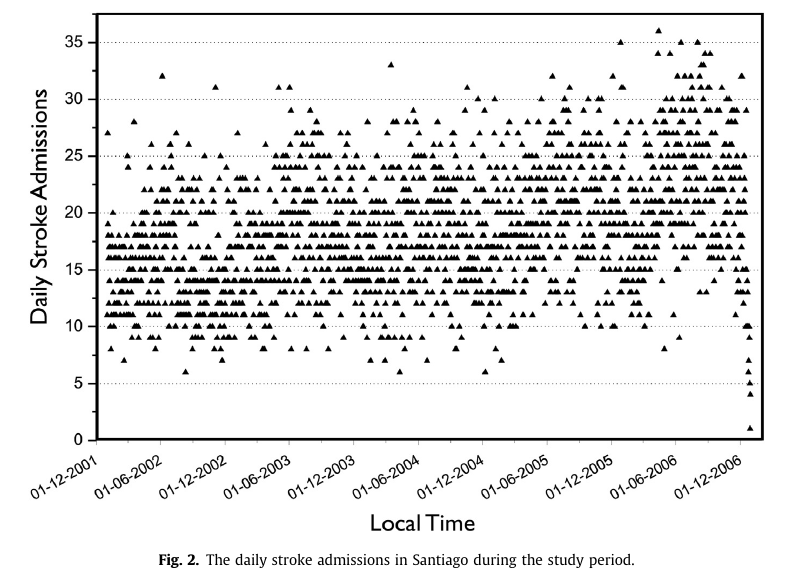
\includegraphics[width=10.92in]{figs/strokes} \caption{Accidentes Cerebro Vasculares Chile (Leiva et al., 2013)}\label{fig:unnamed-chunk-3}
\end{figure}

\hypertarget{impacto-de-las-emisiones-antropogenicas-en-la-calidad-del-aire-y-clima}{%
\chapter{Impacto de las emisiones antropogénicas en la calidad del aire y clima}\label{impacto-de-las-emisiones-antropogenicas-en-la-calidad-del-aire-y-clima}}

La contaminacion es una amenaza a la salud global que causo 9 millones de muertes en 2015, 16\% de las muertes \citep{landrigan2018lancet}. Ademas, existe consenso cientifico de la existencia y relacion con la actividad humana sobre el cambio climatico \citep{cook2016consensus}. Tanto la contaminacion atmosferica como los gases de efecto invernadero, conocidos tambien como forzantes climaticos de vida corta y larga son causados por compuestos quimicos liberados en la atmosfera, las llamadas emisiones. Por lo tanto, es importante realziar y entender la caracterizacion espacial y temporal de las emisiones, asi como sus efectos en la salud y en el clima.

Algunos efectos de la contaminacion atmosferica en la salud

\begin{itemize}
\tightlist
\item
  incrementa la morbilidad, natalidad
\item
  aumenta la tasa de nacimientos con problemas (menos peso, inteligencia)
\item
  incrementa riesgo de cancer
\item
  etc et etc
\end{itemize}

La atmosfera es una delgada capa sobre la tierra, 50\% de su masa esta 5.6 km esta compuestos por varios gases \citep{brasseur2017modeling}, cuya composicion es:

\begin{longtable}[]{@{}ccc@{}}
\toprule
\begin{minipage}[b]{0.15\columnwidth}\centering
Gas\strut
\end{minipage} & \begin{minipage}[b]{0.48\columnwidth}\centering
Razon molar \(mol \cdot mol^{-1}\)\strut
\end{minipage} & \begin{minipage}[b]{0.28\columnwidth}\centering
Principal fuente y comentarios \citep{brasseur1999atmospheric}\strut
\end{minipage}\tabularnewline
\midrule
\endhead
\begin{minipage}[t]{0.15\columnwidth}\centering
Nitrogeno (\(N_2\))\strut
\end{minipage} & \begin{minipage}[t]{0.48\columnwidth}\centering
0.78\strut
\end{minipage} & \begin{minipage}[t]{0.28\columnwidth}\centering
Biologica\strut
\end{minipage}\tabularnewline
\begin{minipage}[t]{0.15\columnwidth}\centering
Oxigeno (\(O_2\))\strut
\end{minipage} & \begin{minipage}[t]{0.48\columnwidth}\centering
0.21\strut
\end{minipage} & \begin{minipage}[t]{0.28\columnwidth}\centering
Biologica\strut
\end{minipage}\tabularnewline
\begin{minipage}[t]{0.15\columnwidth}\centering
Argon (\(A_r\))\strut
\end{minipage} & \begin{minipage}[t]{0.48\columnwidth}\centering
0.0093\strut
\end{minipage} & \begin{minipage}[t]{0.28\columnwidth}\centering
Inerte\strut
\end{minipage}\tabularnewline
\begin{minipage}[t]{0.15\columnwidth}\centering
Dioxido de carbono (\(CO_2\))\strut
\end{minipage} & \begin{minipage}[t]{0.48\columnwidth}\centering
\(400 \cdot10^{-6}\)\strut
\end{minipage} & \begin{minipage}[t]{0.28\columnwidth}\centering
Combustion, oceano, biosfera\strut
\end{minipage}\tabularnewline
\begin{minipage}[t]{0.15\columnwidth}\centering
Neon (\(N_e\))\strut
\end{minipage} & \begin{minipage}[t]{0.48\columnwidth}\centering
\(18 \cdot10^{-6}\)\strut
\end{minipage} & \begin{minipage}[t]{0.28\columnwidth}\centering
Inerte\strut
\end{minipage}\tabularnewline
\begin{minipage}[t]{0.15\columnwidth}\centering
Ozono (\(O_3\))\strut
\end{minipage} & \begin{minipage}[t]{0.48\columnwidth}\centering
\(0.01-10 \cdot10^{-6}\)\strut
\end{minipage} & \begin{minipage}[t]{0.28\columnwidth}\centering
Fotoquimico\strut
\end{minipage}\tabularnewline
\begin{minipage}[t]{0.15\columnwidth}\centering
Helio (\(H_e\))\strut
\end{minipage} & \begin{minipage}[t]{0.48\columnwidth}\centering
\(5.2 \cdot10^{-6}\)\strut
\end{minipage} & \begin{minipage}[t]{0.28\columnwidth}\centering
Inerte\strut
\end{minipage}\tabularnewline
\begin{minipage}[t]{0.15\columnwidth}\centering
Metano (\(CH_4\))\strut
\end{minipage} & \begin{minipage}[t]{0.48\columnwidth}\centering
\(1.8 \cdot10^{-6}\)\strut
\end{minipage} & \begin{minipage}[t]{0.28\columnwidth}\centering
Biogenico y antropogenico\strut
\end{minipage}\tabularnewline
\begin{minipage}[t]{0.15\columnwidth}\centering
Hidrogeno (\(H_2\))\strut
\end{minipage} & \begin{minipage}[t]{0.48\columnwidth}\centering
\(500 \cdot10^{-9}\)\strut
\end{minipage} & \begin{minipage}[t]{0.28\columnwidth}\centering
Biogenico, antropogenico y fotoquimico\strut
\end{minipage}\tabularnewline
\begin{minipage}[t]{0.15\columnwidth}\centering
Oxido nitroso (\(N_2O\))\strut
\end{minipage} & \begin{minipage}[t]{0.48\columnwidth}\centering
\(330 \cdot10^{-9}\)\strut
\end{minipage} & \begin{minipage}[t]{0.28\columnwidth}\centering
Biogenico y antropogenico\strut
\end{minipage}\tabularnewline
\bottomrule
\end{longtable}

\hypertarget{contaminacion-atmosferica---introduccion}{%
\section{Contaminacion atmosferica - Introduccion}\label{contaminacion-atmosferica---introduccion}}

\textbf{``La contaminación del aire es un determinante importante de la salud. La OMS estima que en 2012 alrededor de 1 de cada 8 muertes se atribuyeron a la exposición a la contaminación del aire, lo que lo convierte en el mayor factor de riesgo ambiental para la mala salud.''}\citep{oms}

La ciencia de la contaminacion atmosferica, si bien reciente, ha sido desarrollada debido a los avances de en la comprension de la meteorologia. Problemas relacionados con la contaminacion atmosferica han sido descritos en obras literarias y cartas a lo largo de la historia. Por ejemplo, se cree que el primer caso reportado sobre los efectos de la contaminacion atmosférica en la salud es sobre Gaius Plinius Secundus, Geografo, (AD 23-AD 79), quien habria fallecido los efectos de la \textbf{emisiones} del volcan Vesuvius \citep{art, vis}. La erupcion del volcan Vesuvius duro 19 horas, con altura de lacolumna entre 14 y 32 km y deposicion de material piroplastico de hasta 2500 \(kg \cdot m^{-2}\) \citep{macedonio1988numerical}.

\begin{figure}
\centering
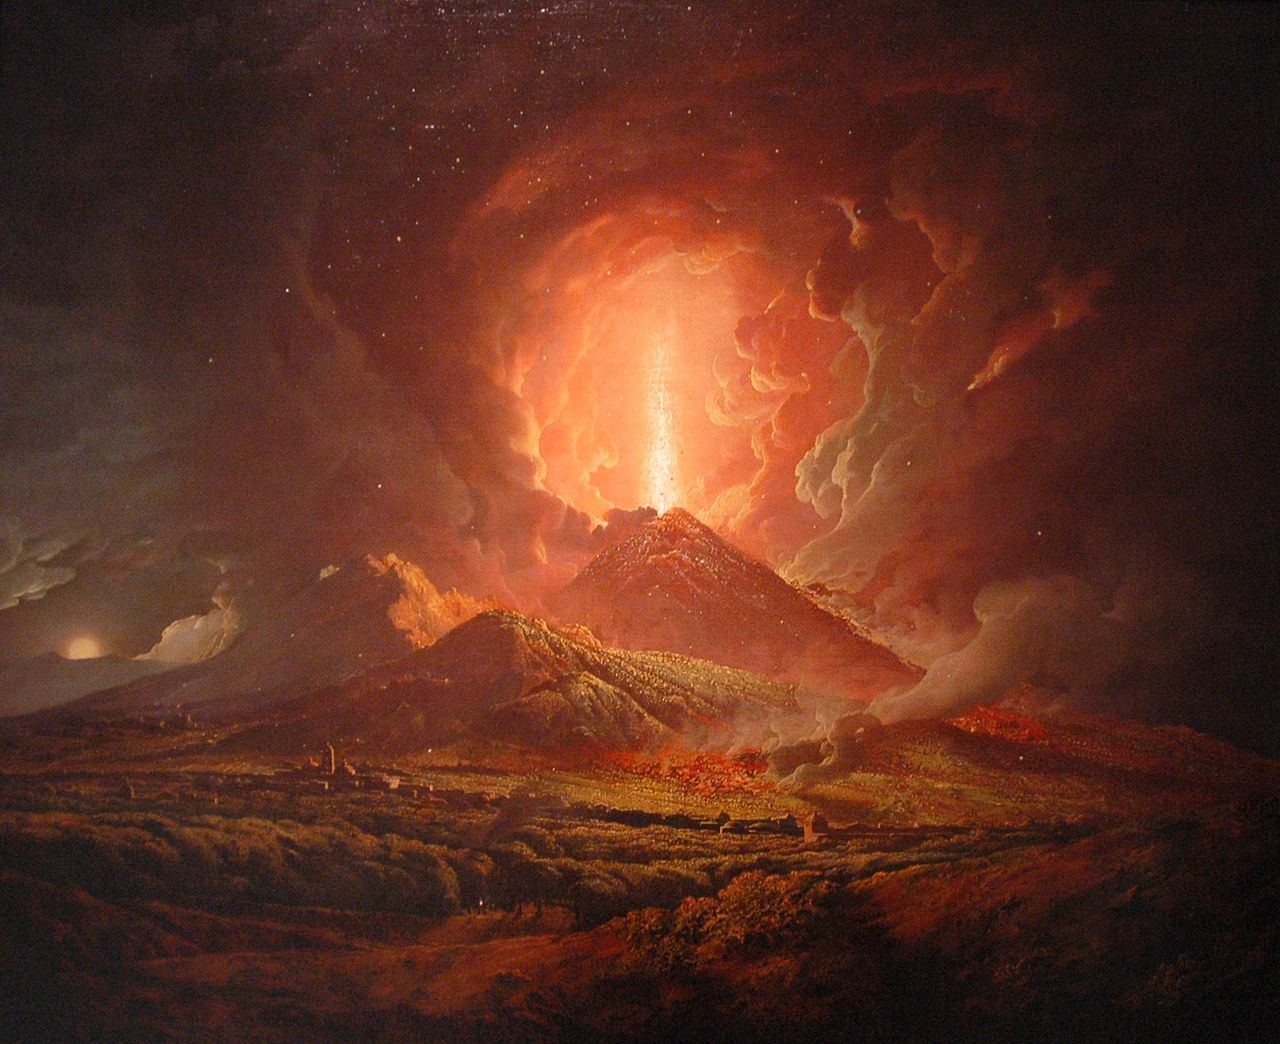
\includegraphics{figs/1280px-Joseph_Wright_of_Derby_-_Vesuvius_from_Portici.jpg}
\caption{\label{fig:unnamed-chunk-4}An eruption of Vesuvius seen from Portici, by Joseph Wright (ca. 1774-6), Dominio Publico}
\end{figure}

Sin embargo han sido los grandes episodios de contaminacion los que han gatillado su estudio y gestion por parte de los tomadores de decisiones. Entre ellos se pueden mencionar el desastre de Londres 1952 y la acidifacion de los lagos escandinavos.

\hypertarget{el-desastre-de-londres-1952}{%
\subsection{El desastre de Londres 1952}\label{el-desastre-de-londres-1952}}

Altas concentraciones de contaminantes fueron ocurrieron entre el 5 y 9 de Diciembre de 1952 en Londres, Inglaterra. Para comparacion, vea el monumento ``Columna de Nelson'' en condiciones normales\citep{nelson1}, y el dia de la llamada ``Gran Niebla de Londres''\citep{nelson2}

\begin{figure}
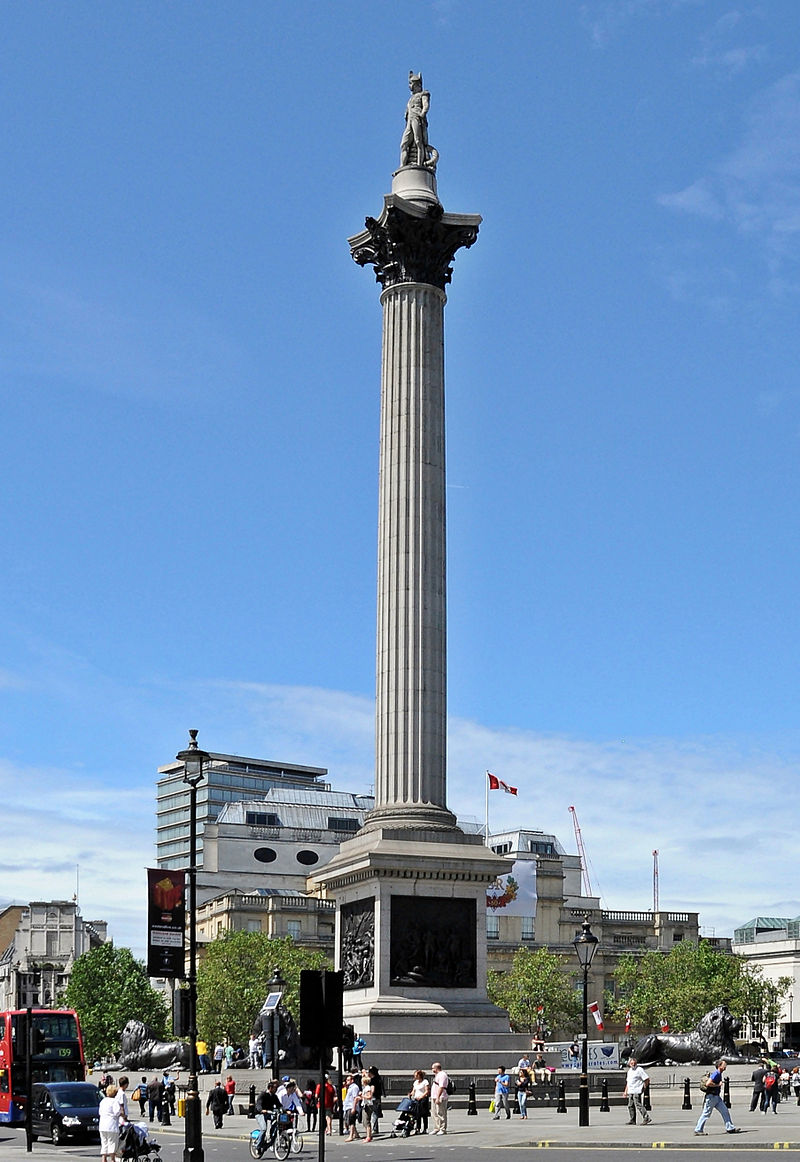
\includegraphics[width=0.9\linewidth,height=0.9\textheight]{figs/800px-Nelson's_Column,_Trafalgar_Square,_London} \caption{Columna de Nelson, Dominio Publico}\label{fig:unnamed-chunk-5}
\end{figure}

\begin{figure}
\centering
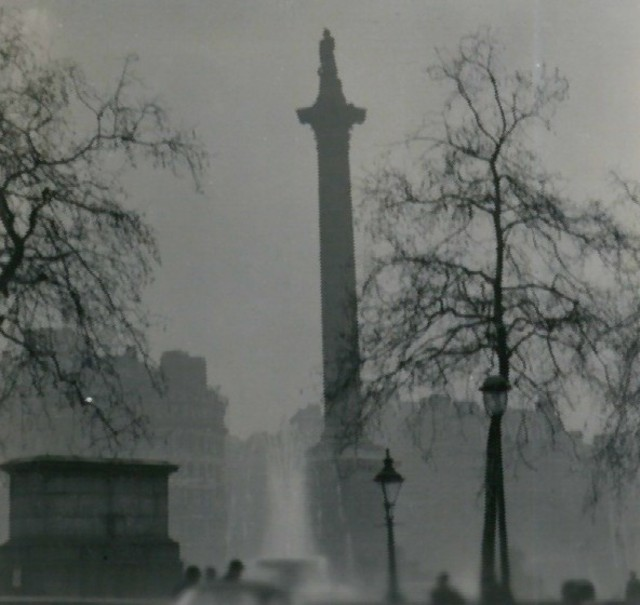
\includegraphics{figs/Nelson's_Column_during_the_Great_Smog_of_1952.jpg}
\caption{\label{fig:unnamed-chunk-6}Columna de Nelson durante la Gran Niebla de 1952, Dominio Publico}
\end{figure}

\hypertarget{consecuencias}{%
\subsubsection{Consecuencias}\label{consecuencias}}

A pesar que durante la fecha, las autoridades no consideraron el efecto de la contaminacion, este evento si causoo gran impacto en la comunidad \citep{l1952}. Estudios posteriores cuantificaron un impacto en \textbf{12.000 muertos} asociados a este episodio de contaminacion \citep{bell2001reassessment}.

\begin{figure}
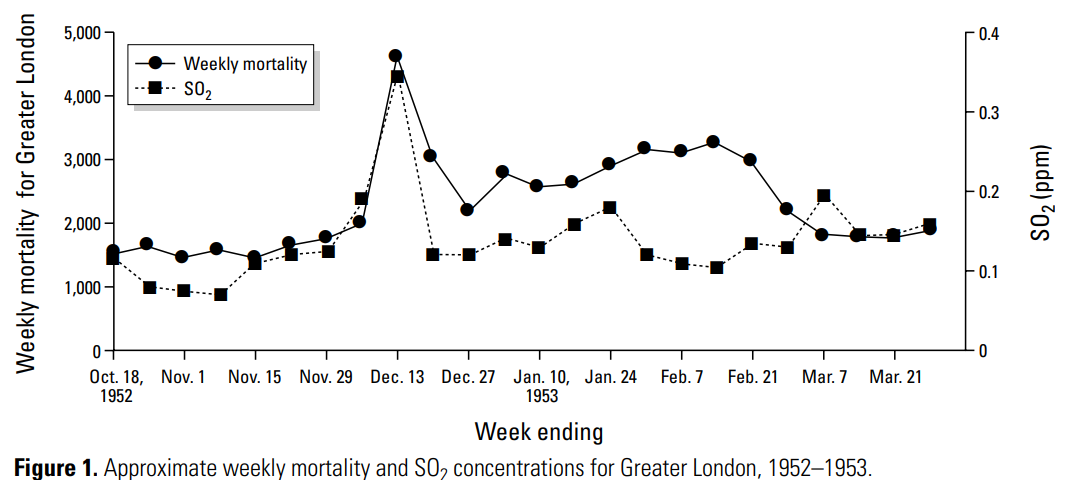
\includegraphics[width=1.2\linewidth]{figs/so2lon} \caption{Mortalidad semanal y concentraciones de SO2 en Lobres 1952 (Bell and Davis, 2001)}\label{fig:unnamed-chunk-7}
\end{figure}

\begin{figure}
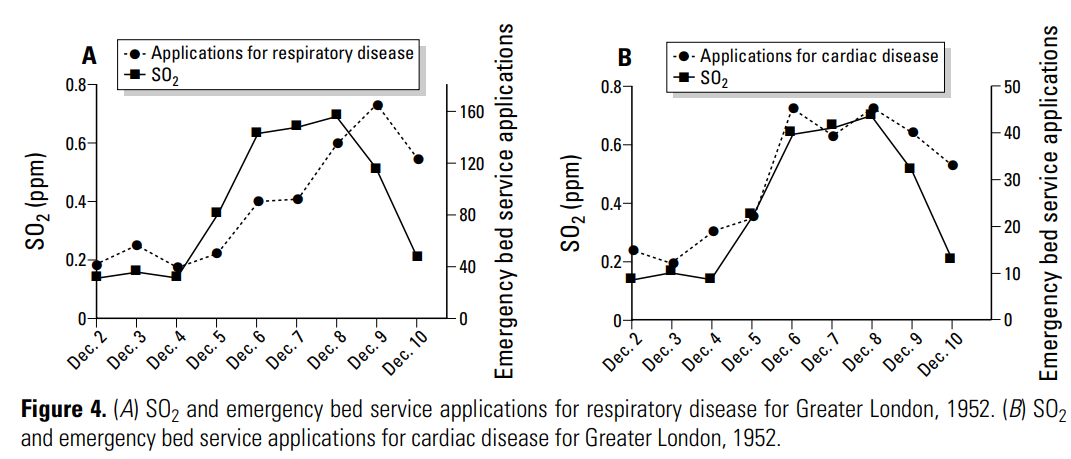
\includegraphics[width=1.2\linewidth]{figs/so2lon2} \caption{Mortalidad semanal y concentraciones de SO2 en Lobres 1952 (Bell and Davis, 2001)}\label{fig:unnamed-chunk-8}
\end{figure}

\emph{comentarios?}

\hypertarget{clrtap}{%
\subsubsection{CLRTAP}\label{clrtap}}

\begin{verbatim}
## Tarea / Tema de casa / Homework:
\end{verbatim}

\begin{verbatim}
## [1] "Investique que es, causas, consequencias y poltiica ambiental asociada a CLRTAP"
\end{verbatim}

\hypertarget{contaminantes-atmosfericos}{%
\section{Contaminantes atmosfericos}\label{contaminantes-atmosfericos}}

Las emisiones liberadas a la atmosfera impactan la salud, meteorologia y clima en diferentes escalas como se ve en la sigueinte figura.

\begin{figure}
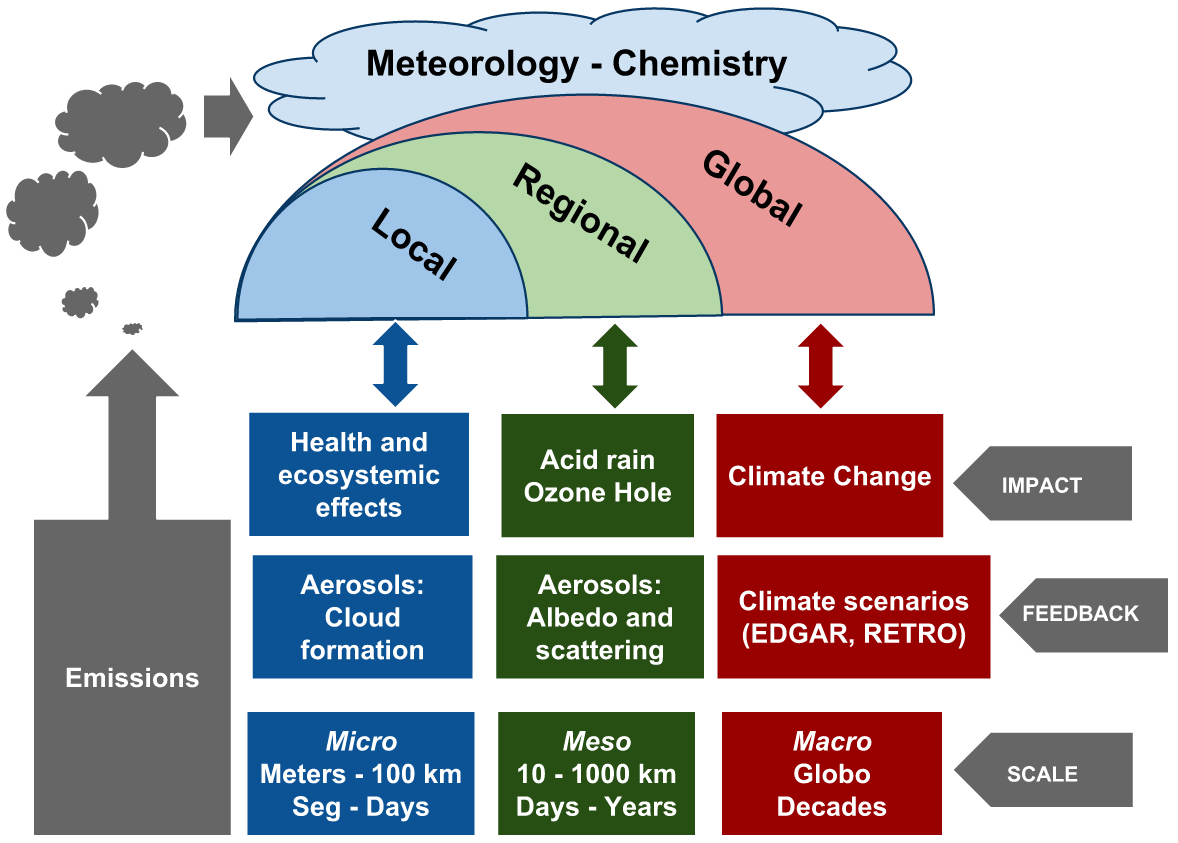
\includegraphics[width=1.3\linewidth]{figs/esquema} \caption{Esquema de impacto de emisiones (Ibarra, 2017)}\label{fig:unnamed-chunk-10}
\end{figure}

Por lo tanto para entender las emisiones necesitamos respnder las siguientes preguntas:

\begin{itemize}
\tightlist
\item
  \textbf{Que?}
\item
  \textbf{Como?}
\item
  \textbf{Cuando?}
\item
  \textbf{Donde?}
\end{itemize}

Los contaminantes atmosfericos suelen ser clasificados como:

\begin{itemize}
\tightlist
\item
  Primarios: emitidos directamente en la atmosfera. Ejemplo: CO.
\item
  Secundarios: formados en la atmosfera. Ejemplo: \(O_3\).
\end{itemize}

Existen muchos contaminantes atmosfericos de interes cientifico como

\begin{itemize}
\tightlist
\item
  Ozono \(O_3\)
\item
  Monoxido de Carbono \(CO\)
\item
  Radicales de Oxidos de nitrogeno \(NO_X \equiv NO + NO_2\)
\item
  Compuestos organicos volatiles \(COV\)
\item
  Radicales de Halogeno
\item
  Especies de azufre \(SO_2\), \(SO4\), \(H_2SO_4\)
\item
  Aersoles
\end{itemize}

\textbf{Cada contaminante tiene un extenso cuerpo teorico. En esta parte del curso nos referiremos brevemente al \(O_3\), aerosoles y especies de azufre, sin embargo, el estudiante puede revisar la bibliografia para se aprofundar.}

\hypertarget{ozono-o_3}{%
\subsection{\texorpdfstring{Ozono \(O_3\)}{Ozono O\_3}}\label{ozono-o_3}}

Respecto del ozono es necesario mencionar que existen dos tipos, el estratosferico (bueno) y y el troposferico (malo),
como es expicado por \citet{brasseur2017modeling}.

El ciclo deo ozono troposferico comienza con la fotolisis de lamolecula de ox{[}igeno devido a radiacion solar de longitud de onda minimo 242 nm. Posteriormente, un atomo de oxigeno se combina con otra molecula de oxigeno para formar ozono. La molecula M (cuerpo inerte, como \(N_2\) o \(O_2\)) estabiliza la molecula de \(O_3\) recien formada.

\begin{equation}
O_2 + hv(\lambda < 242 nm)  \rightarrow O + O 
\label{eq:1}
\end{equation}

\begin{equation}
O + O_2 + M     \rightarrow O_3 + M 
\label{eq:2}
\end{equation}

El Ozono luego es fotolizado a un atomo de oxigeno y una molecula de oxigeno ante radiacion menor a 1180 nm, liberando energia cinetica \citep{o3}.

En el caso del ozono troposfeico, la reaccion comienza quando el \href{https://en.wikipedia.org/wiki/Hydroxyl_radical}{radical hidroxilo} \(\cdot OH\) oxida el \(CO\) generando el radical \(\cdot HOCO\) que es inestable y reacciona rapidamente con \(O_2\) generando el \href{https://en.wikipedia.org/wiki/Hydroperoxyl}{peroxi radical} \(\cdot HO_2\) y \(CO_2\). El peroxi radical reacciona oxida \(NO\) generando \(NO_2\) y un radical hidroxilo. Luego el \(NO_2\) es fotolizado liberando un atomo de oxigeno que reacciona con la molecula de \(O_2\) generando \(O_3\).

\begin{equation}
O_3 + hv(\lambda < 1180 nm)     \rightarrow O + O_2 + energia cinetica 
\label{eq:3}
\end{equation}

En el caso del ozono troposferico, los ingredientes principales son radiacion solar, \(NO_x\) y compuestos organicos volatiles \citep{o3wiki}.

\begin{equation}
\cdot OH + CO   \rightarrow \cdot HOCO
\label{eq:4}
\end{equation}

\begin{equation}
\cdot HOCO + O_2    \rightarrow HO_2\cdot + CO_2
\label{eq:5}
\end{equation}

\begin{equation}
HO_2\cdot + NO  \rightarrow \cdot OH + NO_2
\label{eq:6}
\end{equation}

\begin{equation}
NO_2 + hv(\lambda < 400nm)  \rightarrow NO + O
\label{eq:7}
\end{equation}

\begin{equation}
O + O_2     \rightarrow O_3
\label{eq:8}
\end{equation}

Los mecanismos mostrados son un resumen de complejas reacciones en la atmosfera donde muchas otras reacciones y compuestos juegan un rol.

\hypertarget{especies-de-azufre}{%
\subsection{Especies de azufre}\label{especies-de-azufre}}

El es un compuesto que reacciona generando importantes contaminantes como sulfatos y acido sulfurico, importantesen la lluvia aida (deposicion acida). Los combustibles tienen azufre y durante la combustion, el azufre es oxidado generando \(SO_2\), diesel tiene mayor cantidad de azufre que gasolina, por lo tanto generando mas \(SO_2\). Tambien existe el dimetilsulfido (DMS) \((CH3)_2S\), que es biogenico, asi como el carbonilo sulfido (COS), que largo tiempo de vida que permite su transporte a la estratosfera. A continuacion una resumen de los mecanismos de generacion de acido sulfurico \citep{brasseur2017modeling}. \(SO_2\) es oxiado por \(OH\)

\begin{equation}
SO_2 + OH + M   \rightarrow HSO_3 + M
\label{eq:9}
\end{equation}

\begin{equation}
HSO_3 + O_2     \rightarrow  SO_3 + HO_2
\label{eq:10}
\end{equation}

\begin{equation}
SO_3 + H2O + M \rightarrow  H_2SO_4 + M
\label{eq:11}
\end{equation}

\hypertarget{aerosoles}{%
\subsection{Aerosoles}\label{aerosoles}}

Son particulas suspendidas desde \textasciitilde{}0.001 \(\mu m\) hasta 100 \(\mu m\) (luster molecular a gota). Conocido como material particulado (MP), sus caracerizacion es realizada mayormente en base a su diametro aerodinamico como se muestra en la sigueinte figura \citep{mpwiki}\citep{brasseur2017modeling}. Existen tres agrupaciones que son:

\begin{enumerate}
\def\labelenumi{\arabic{enumi}.}
\tightlist
\item
  Modo Aiken: nucleos de condensacion nuevos (fresh) que condensan (gas) o coagulan (liquidos). Diametro hasta 100 nm.
\item
  Modo acumulacion: Diametro entre 100 y 1000 nm.
\item
  Modo coarse: Diametro mayor que 1000 nm.
\end{enumerate}

\begin{figure}
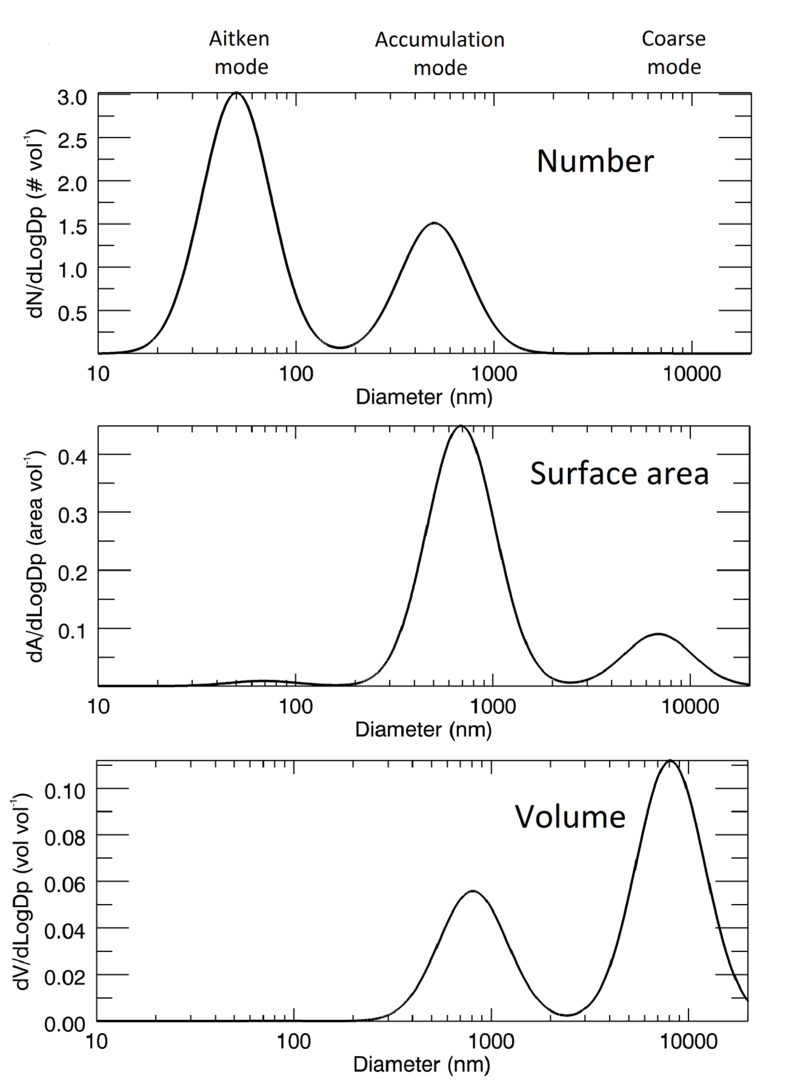
\includegraphics[width=1.2\linewidth]{figs/800px-Synthetic_aerosol_distribution_in_number_area_and_volume_space} \caption{Distribucion normalizada (suma es 1000) de aerosoles por diametro aerodinamico, Dominio Publico}\label{fig:unnamed-chunk-11}
\end{figure}

Los aersolos son claisficados por numeros, area de superficie y volumen. Normalmente las agencias de medio ambiente miden \(MP_{10}\) (diametro menos \textless{}= que 10 \(\mu m\)) y \(MP_{2.5}\) (diametro menos \textless{}= que 2.5 \(\mu m\)) en \(\mu g \cdot m^{-3}\). A continuacion una figura mostrando material particulado en Chile, Brazil y China.

\textbf{Chile }*

\begin{figure}
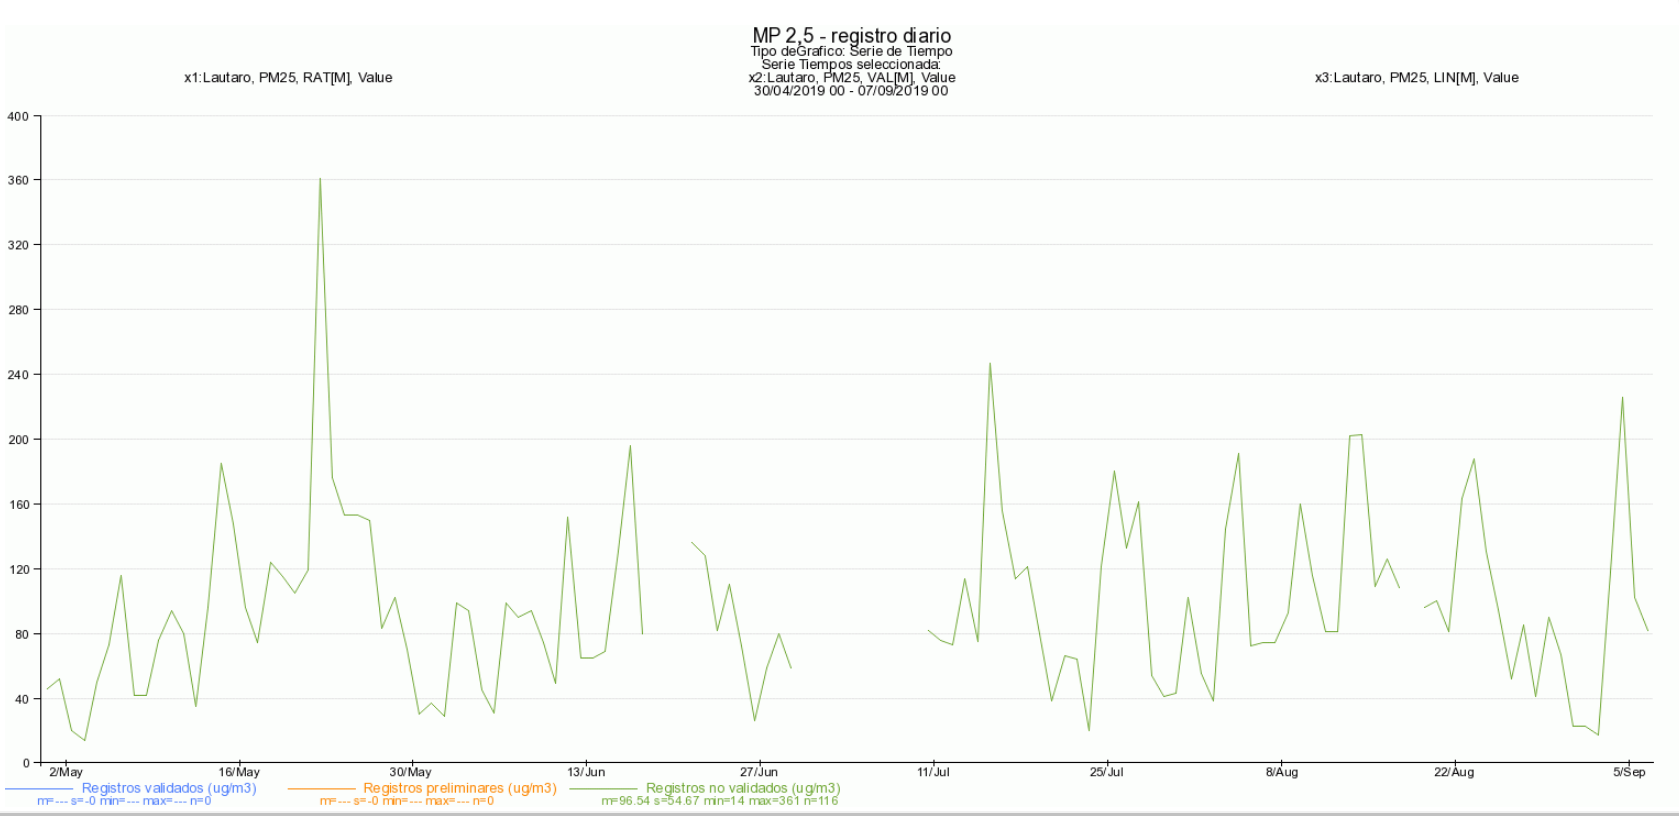
\includegraphics[width=23.32in]{figs/chile1} \caption{MP2.5 ug/m3 em Lautaro, Chile (https://sinca.mma.gob.cl/index.php/estacion/index/key/870)}\label{fig:unnamed-chunk-12}
\end{figure}

\textbf{China}

\begin{figure}
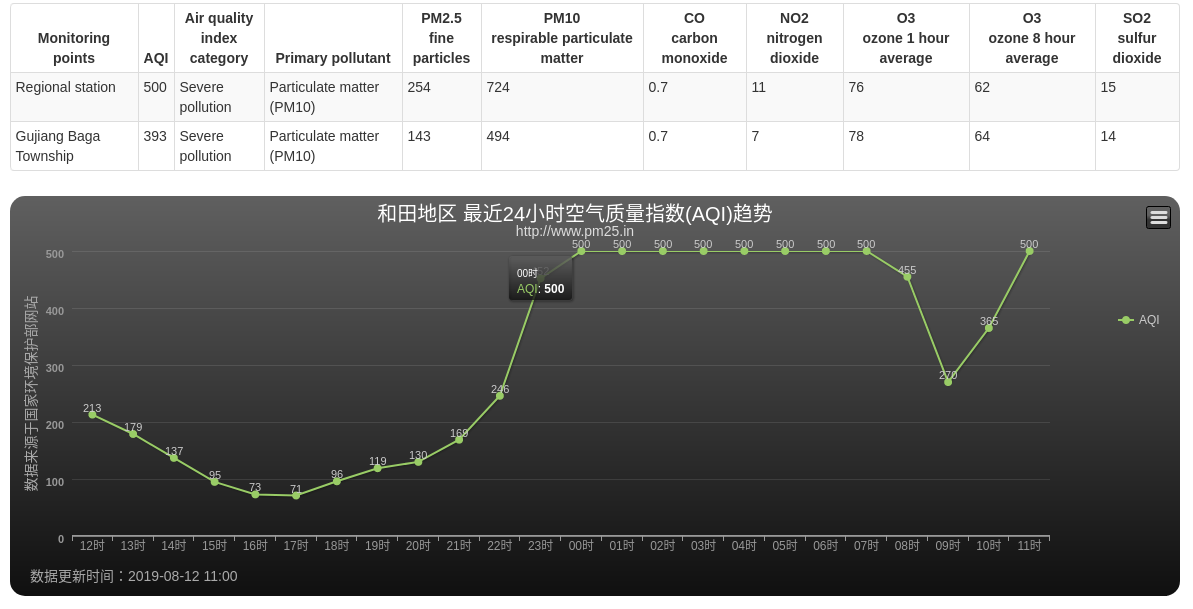
\includegraphics[width=1.5\linewidth]{figs/hotan} \caption{MP2.5 ug/m3 em Hotan, China (http://pm25.in/hetiandiqu)}\label{fig:unnamed-chunk-13}
\end{figure}

ingrese aqui: \url{https://aqicn.org/forecast/beijing/}

\textbf{Osasco, Brasil}

\begin{figure}
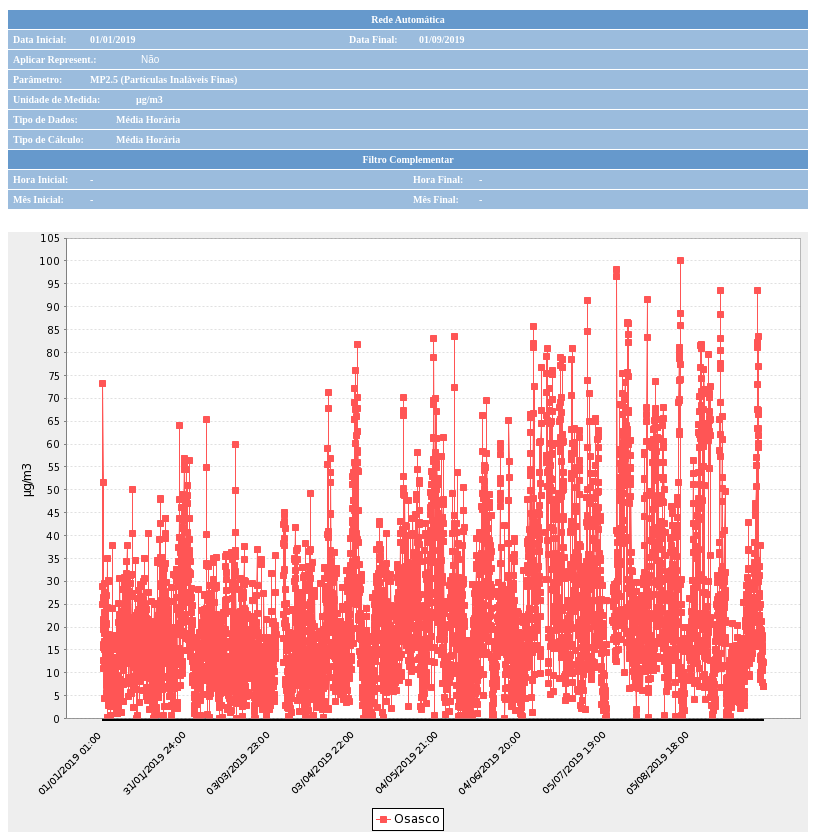
\includegraphics[width=1.5\linewidth]{figs/brazil} \caption{MP2.5 ug/m3 Osasco, Brasil (https://qualar.cetesb.sp.gov.br)}\label{fig:unnamed-chunk-14}
\end{figure}

\href{https://worldview.earthdata.nasa.gov/}{NASA WORLDVIEW} es un excelente recurso para monitorear aerosoles, incendios y mucho mas.

\begin{verbatim}
## Ingrese a https://worldview.earthdata.nasa.gov/ y busque aerosol
\end{verbatim}

\hypertarget{forzantes-climaticos-y-gases-de-efecto-invernadero}{%
\section{Forzantes climaticos y gases de efecto invernadero}\label{forzantes-climaticos-y-gases-de-efecto-invernadero}}

El efecto invernadero es un fenomeno que e produce naturalmente en la tierra, sin intervencion humana. Por ejemplo, concentraciones biogenicas de CO2 o el vapor de agua. Sin embargo, el termino forzante climatico se refiere de estos compuestos quimicos tienen una incidencia en el clima, pues alteran el cambio en iradiancia neta \(W \cdot m^{-2}\).

El forzante radiativo es utilizado como predictor de cambio en la media global de temperatura. IPCC \citep{schimel1996radiative} define forzamiento radiativo como:

``The radiative forcing of the surface-troposphere system due to the perturbation in or the introduction of an agent
(say, a change in greenhouse gas concentrations) is the change in net (down minus up) irradiance (solar plus long-wave; in Wm−2) at the tropopause AFTER allowing for stratospheric temperatures to readjust to radiative equilibrium, but with surface and tropospheric temperatures and state held fixed at the unperturbed values'' \citep{schimel1996radiative}

Del sitio web de Copernicus (\url{https://atmosphere.copernicus.eu/climate-forcing}:

``Climate forcing measures the imbalance in the Earth's energy budget caused by a perturbation of the climate system, for example changes in atmospheric composition driven by human activities. \textbf{Climate forcing, also known as Radiative Forcing, therefore determines the change in globally-averaged temperature change due to the natural or human-induced changes to the energy budget}. Increases in greenhouse gas concentrations over the industrial era are responsible for a positive climate forcing, causing a gain of energy in the climate system. In contrast, changes in atmospheric aerosol concentrations result in a negative climate forcing leading to a loss of energy. It is the balance between these various climate forcings that drive the change in global temperature.'' \url{https://atmosphere.copernicus.eu/climate-forcing}

\begin{figure}
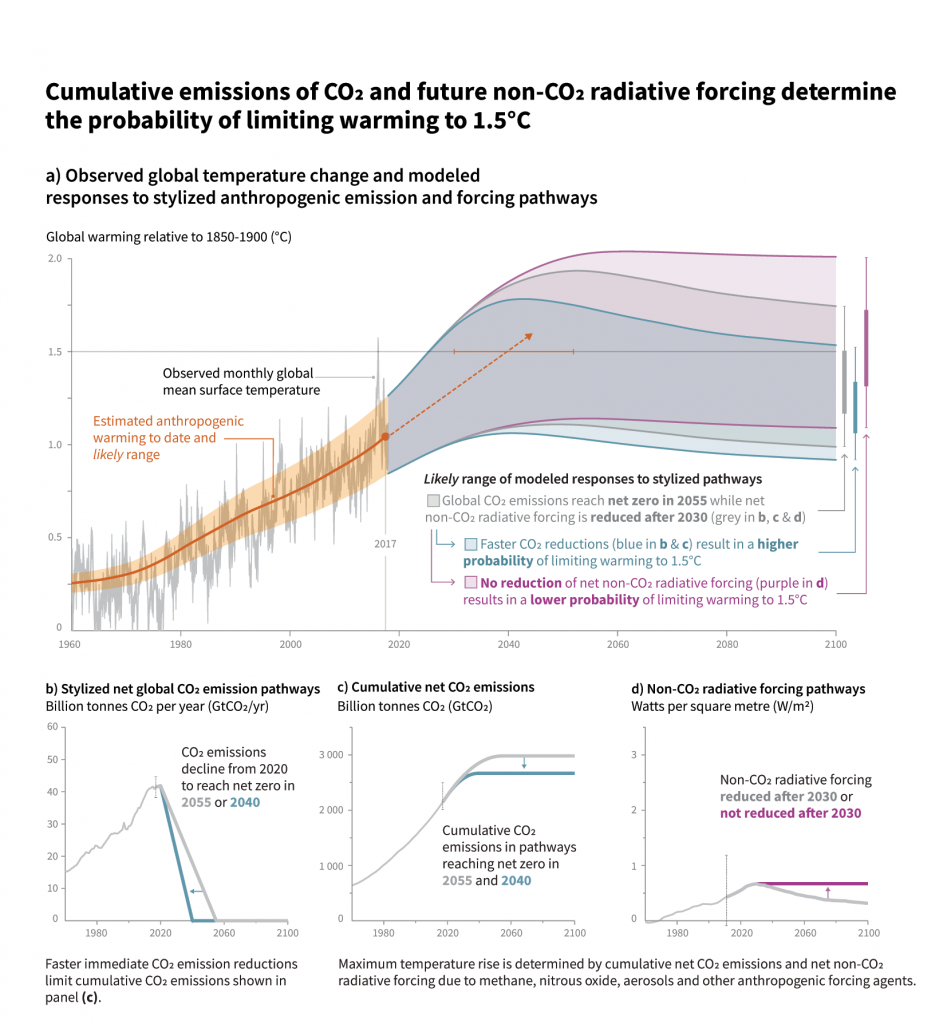
\includegraphics[width=1.2\linewidth]{figs/SPM1_figure-final-947x1024} \caption{Cambio en la temperatura media debido a forzantes radiativas (https://atmosphere.copernicus.eu/climate-forcing)}\label{fig:unnamed-chunk-16}
\end{figure}

\begin{figure}
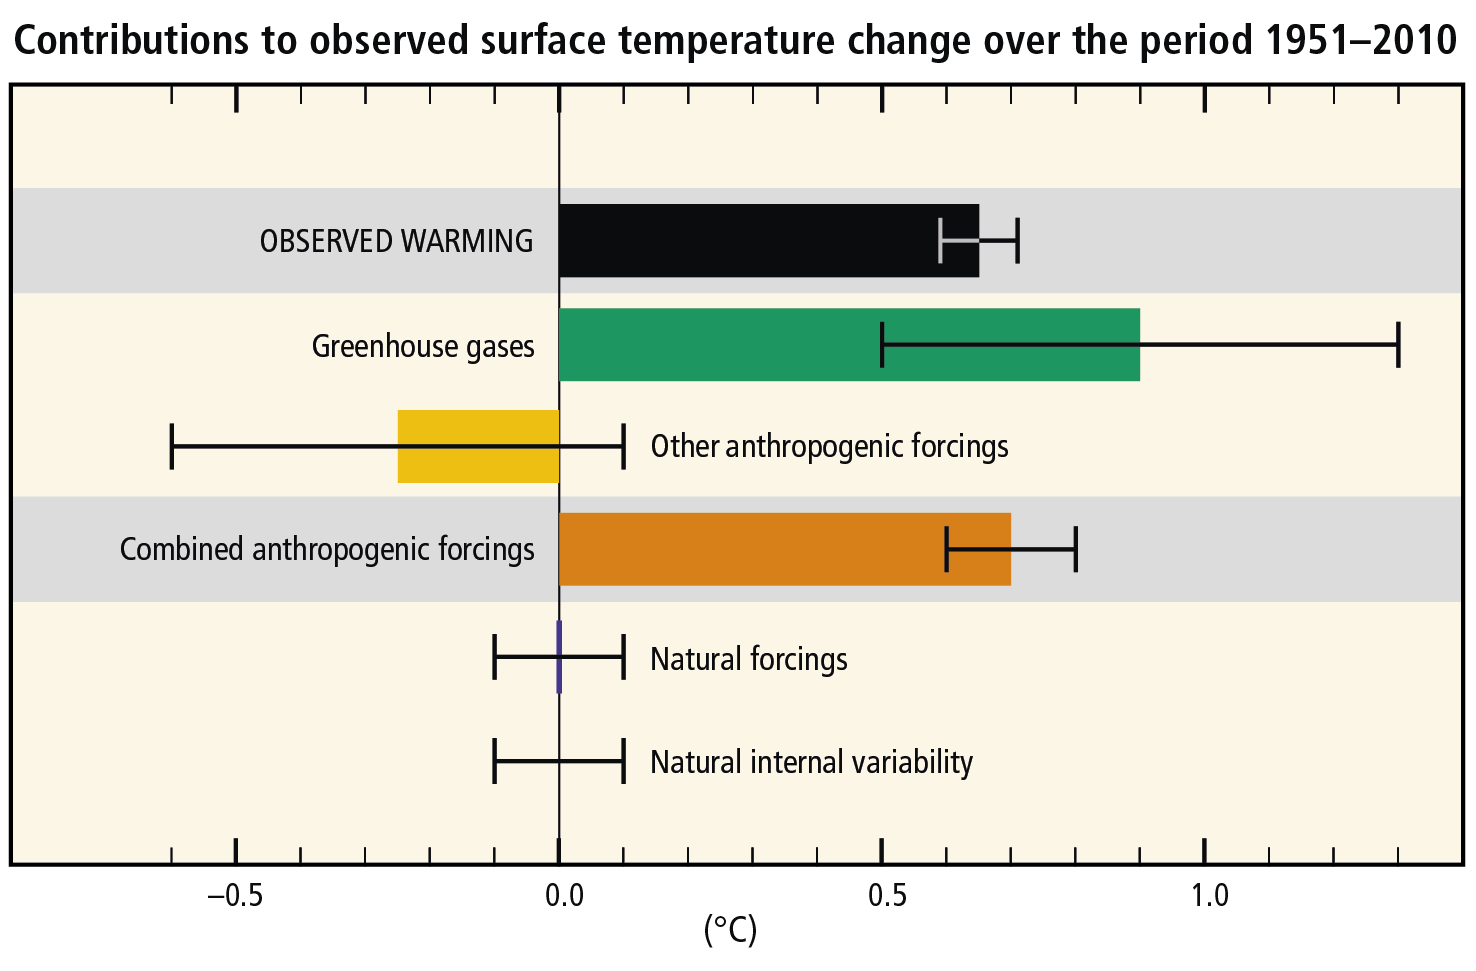
\includegraphics[width=20.5in]{figs/SPM.03-01} \caption{Cambio en la temperatura media debido a forzantes radiativas (https://atmosphere.copernicus.eu/climate-forcing)}\label{fig:unnamed-chunk-17}
\end{figure}

Esta figura muestra un resumen de los compuestos y su forzante radiativo (FR) \citep{stocker2014climate}

\begin{figure}
\centering
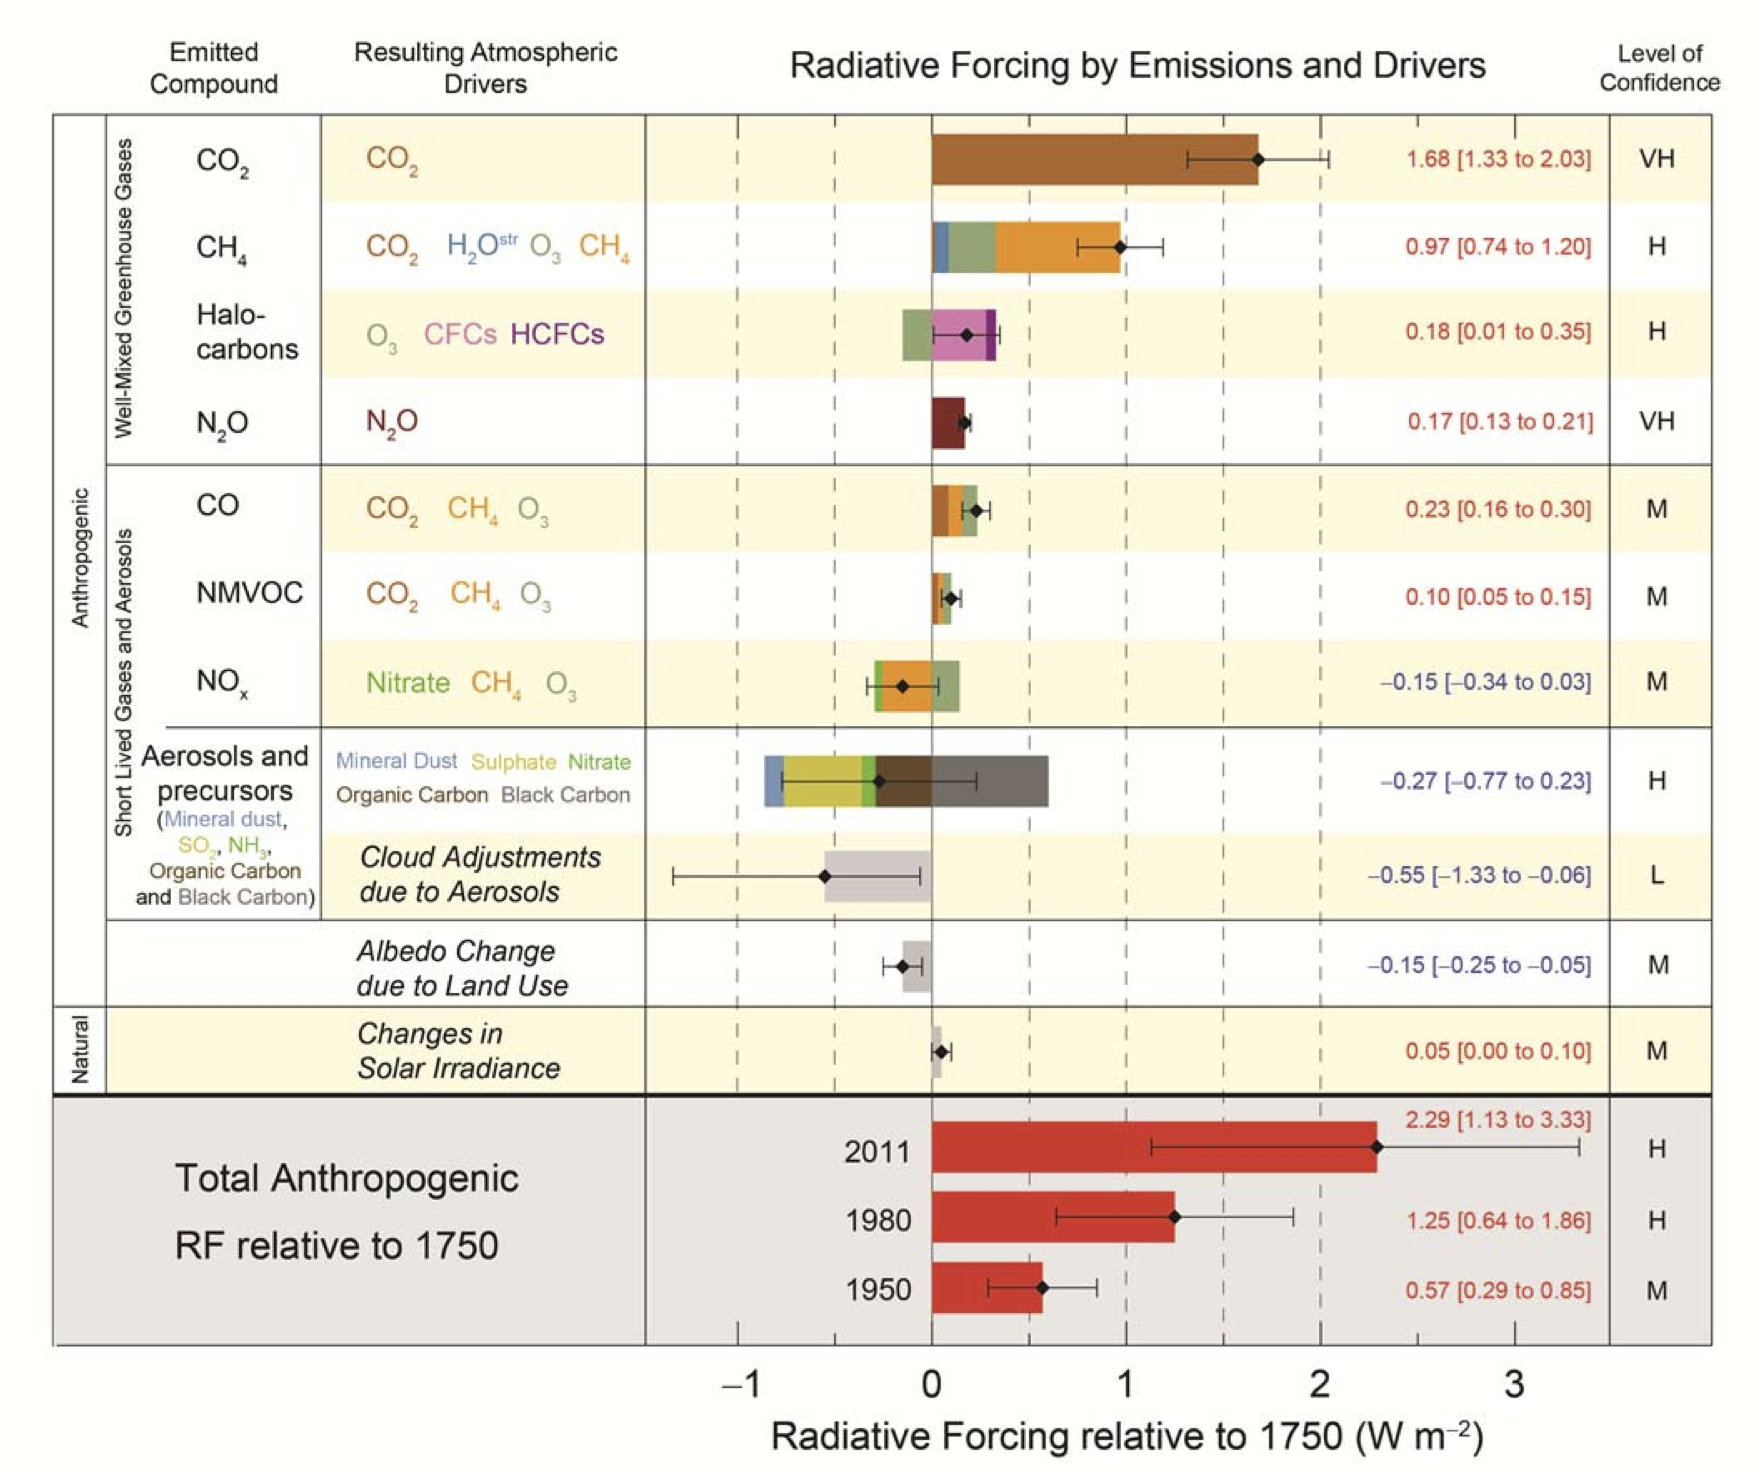
\includegraphics{figs/ipcc.jpg}
\caption{\label{fig:unnamed-chunk-18}Forzante radiativo (\url{https://atmosphere.copernicus.eu/climate-forcing})}
\end{figure}

\hypertarget{efectos-directos-e-indirectos-de-aerosoles}{%
\subsection{Efectos directos e indirectos de aerosoles}\label{efectos-directos-e-indirectos-de-aerosoles}}

\begin{itemize}
\tightlist
\item
  Directo: Influencia en balance radiativo.
\item
  Indirecto: Influencia en el climia.
\item
  Primer efecto indirecto: microfisica de la precipitacion.
\item
  Segundo efecto indirecto: Cantidad de lluvia.
\end{itemize}

\textbackslash{}begin\{figure\}
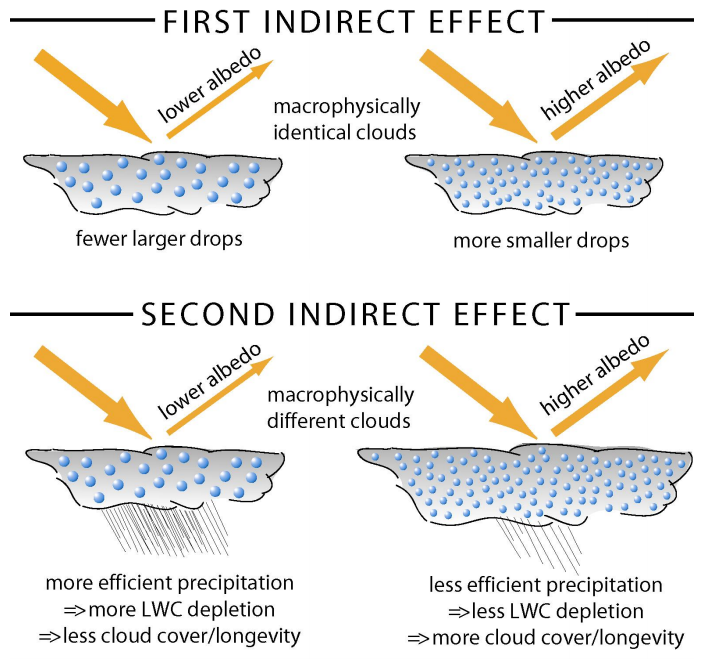
\includegraphics[width=1.1\linewidth]{figs/fx} \textbackslash{}caption\{Forzantes indirectos (Robwood, 2019) (\url{https://atmos.uw.edu/~robwood/teaching/591/ATMS_591_Albrecht_1989.pdf})\}\label{fig:unnamed-chunk-19}
\textbackslash{}end\{figure\}

\hypertarget{black-carbon---carbono-negro}{%
\subsection{Black Carbon - Carbono negro}\label{black-carbon---carbono-negro}}

Son particulas producto de la combustion incompleta de combustibles con origen antropogenico y biogenico.
Considerado el segundo gas de efecto invernadero despues de CO2 \citep{bond2013bounding}.

\begin{figure}
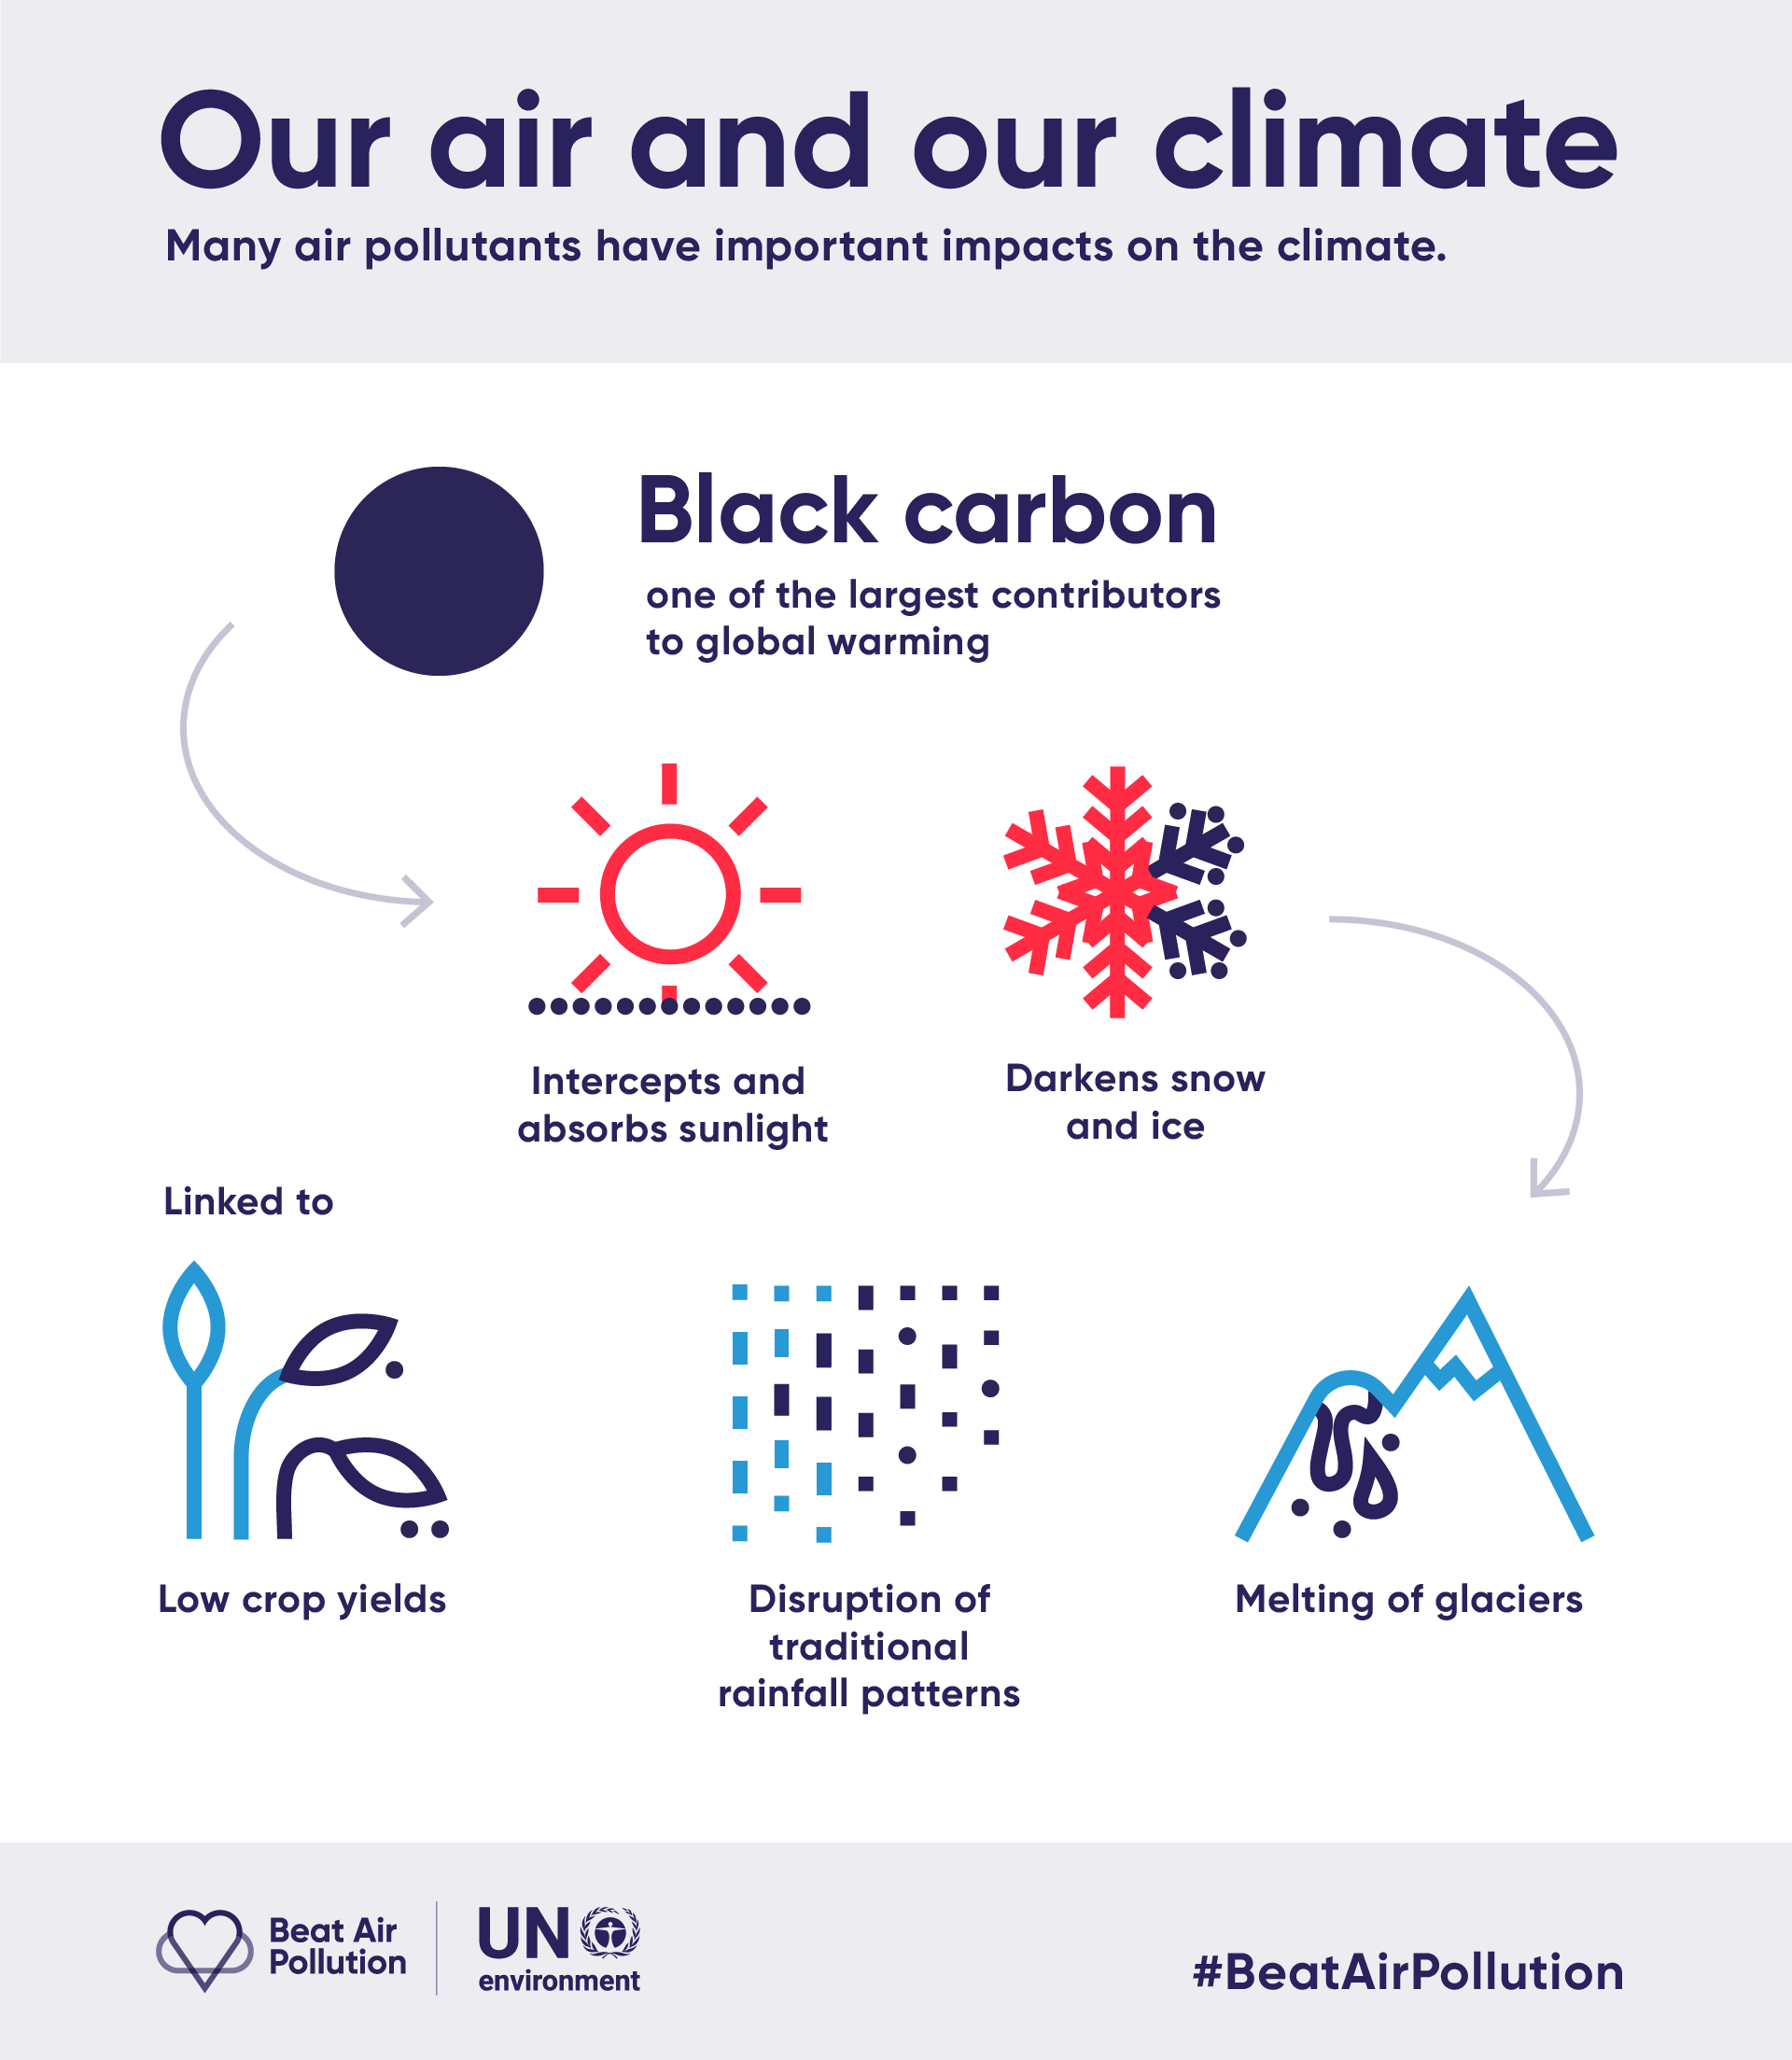
\includegraphics[width=0.9\linewidth]{figs/bc} \caption{UNEP (https://twitter.com/UNEnvironment/status/1150404638501416961/photo/1}\label{fig:unnamed-chunk-20}
\end{figure}

\hypertarget{emisiones-y-sus-fuentes}{%
\section{Emisiones y sus fuentes}\label{emisiones-y-sus-fuentes}}

Un inventario de emisiones es la compilacion del flujo de masa de contaminantes emitida en un lugar y tiempo determinado.

Son definidos por la ecuacion basica de :

\begin{equation}
E = FE \cdot NA
\label{eq:12}
\end{equation}

Donde E es la emision, FE es el factor de emision y NA el nivel de actividad. Por ejemplo, si queremos saber las emisiones de vehiculos, FE esta en \textbf{g/km}, NA es la cantidad de vehiculos veces la distancia que recorren \textbf{km} en un tiempo determinado, luego E es la masa \textbf{g} de contaminantes.

\hypertarget{tipos}{%
\subsection{Tipos}\label{tipos}}

Ya que ya sabemos los contaminantes y su forzamiento radiativo, podemos ver cuales son las fuentes de ellos, desde elpunto de vista de contaminacion atmosferica y clima. Existen varios tipos de fuentes de emisiones:

\begin{figure}
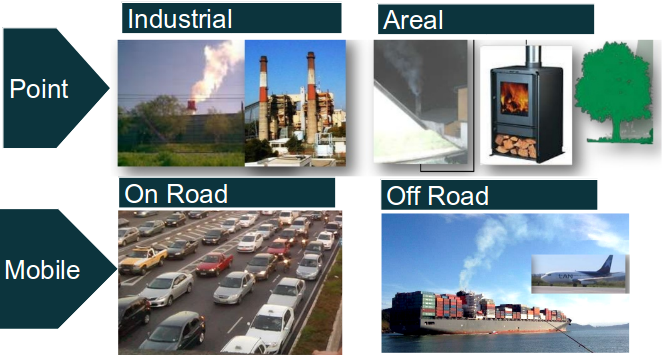
\includegraphics[width=1.3\linewidth]{figs/fuentes} \caption{Fuentes de emisiones}\label{fig:unnamed-chunk-21}
\end{figure}

Pueden tener aplicaciones de gestion y cientificas:

\begin{figure}
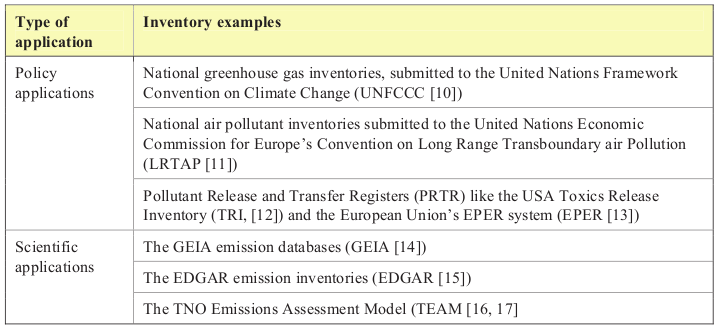
\includegraphics[width=1.5\linewidth]{figs/theart2} \caption{Tipos de inventarios (Pules and Helsinga, 2013)}\label{fig:unnamed-chunk-22}
\end{figure}

Por ejemplo, IPCC entrega guias para que los paises compilen inventarios de emisiones de gases de fecto invernadero:

\begin{figure}
\centering
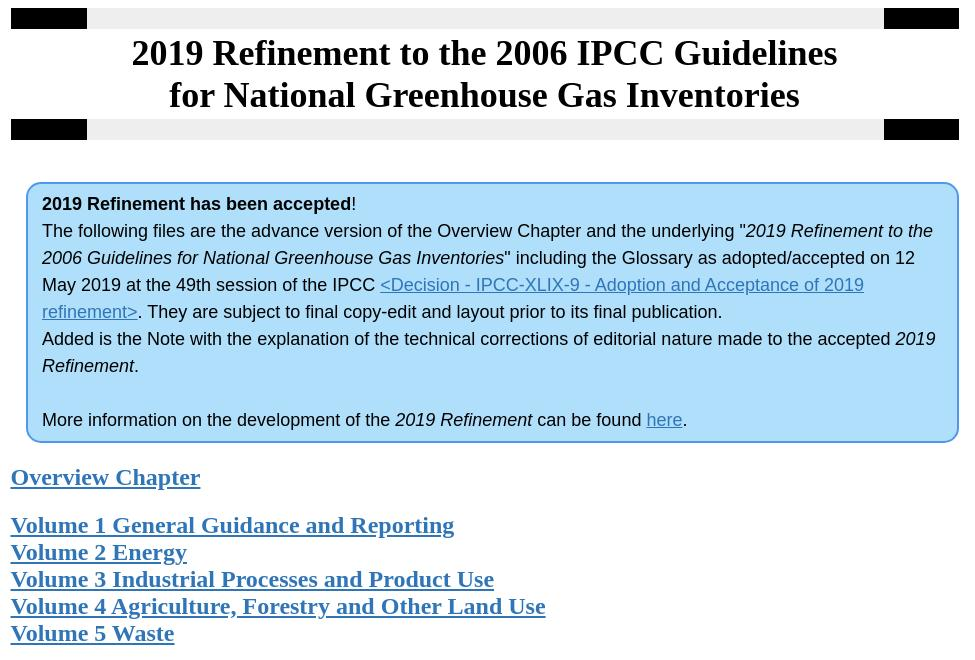
\includegraphics{figs/ipcc2.jpg}
\caption{\label{fig:unnamed-chunk-23}Actualizacion en las guias de inventarios de emisiones IPCC (\url{https://www.ipcc-nggip.iges.or.jp/public/2019rf/index.html})}
\end{figure}

Ahora podemos ver como ha sido la serie de emisiones globales de gases de efecto invernadero:

\begin{figure}
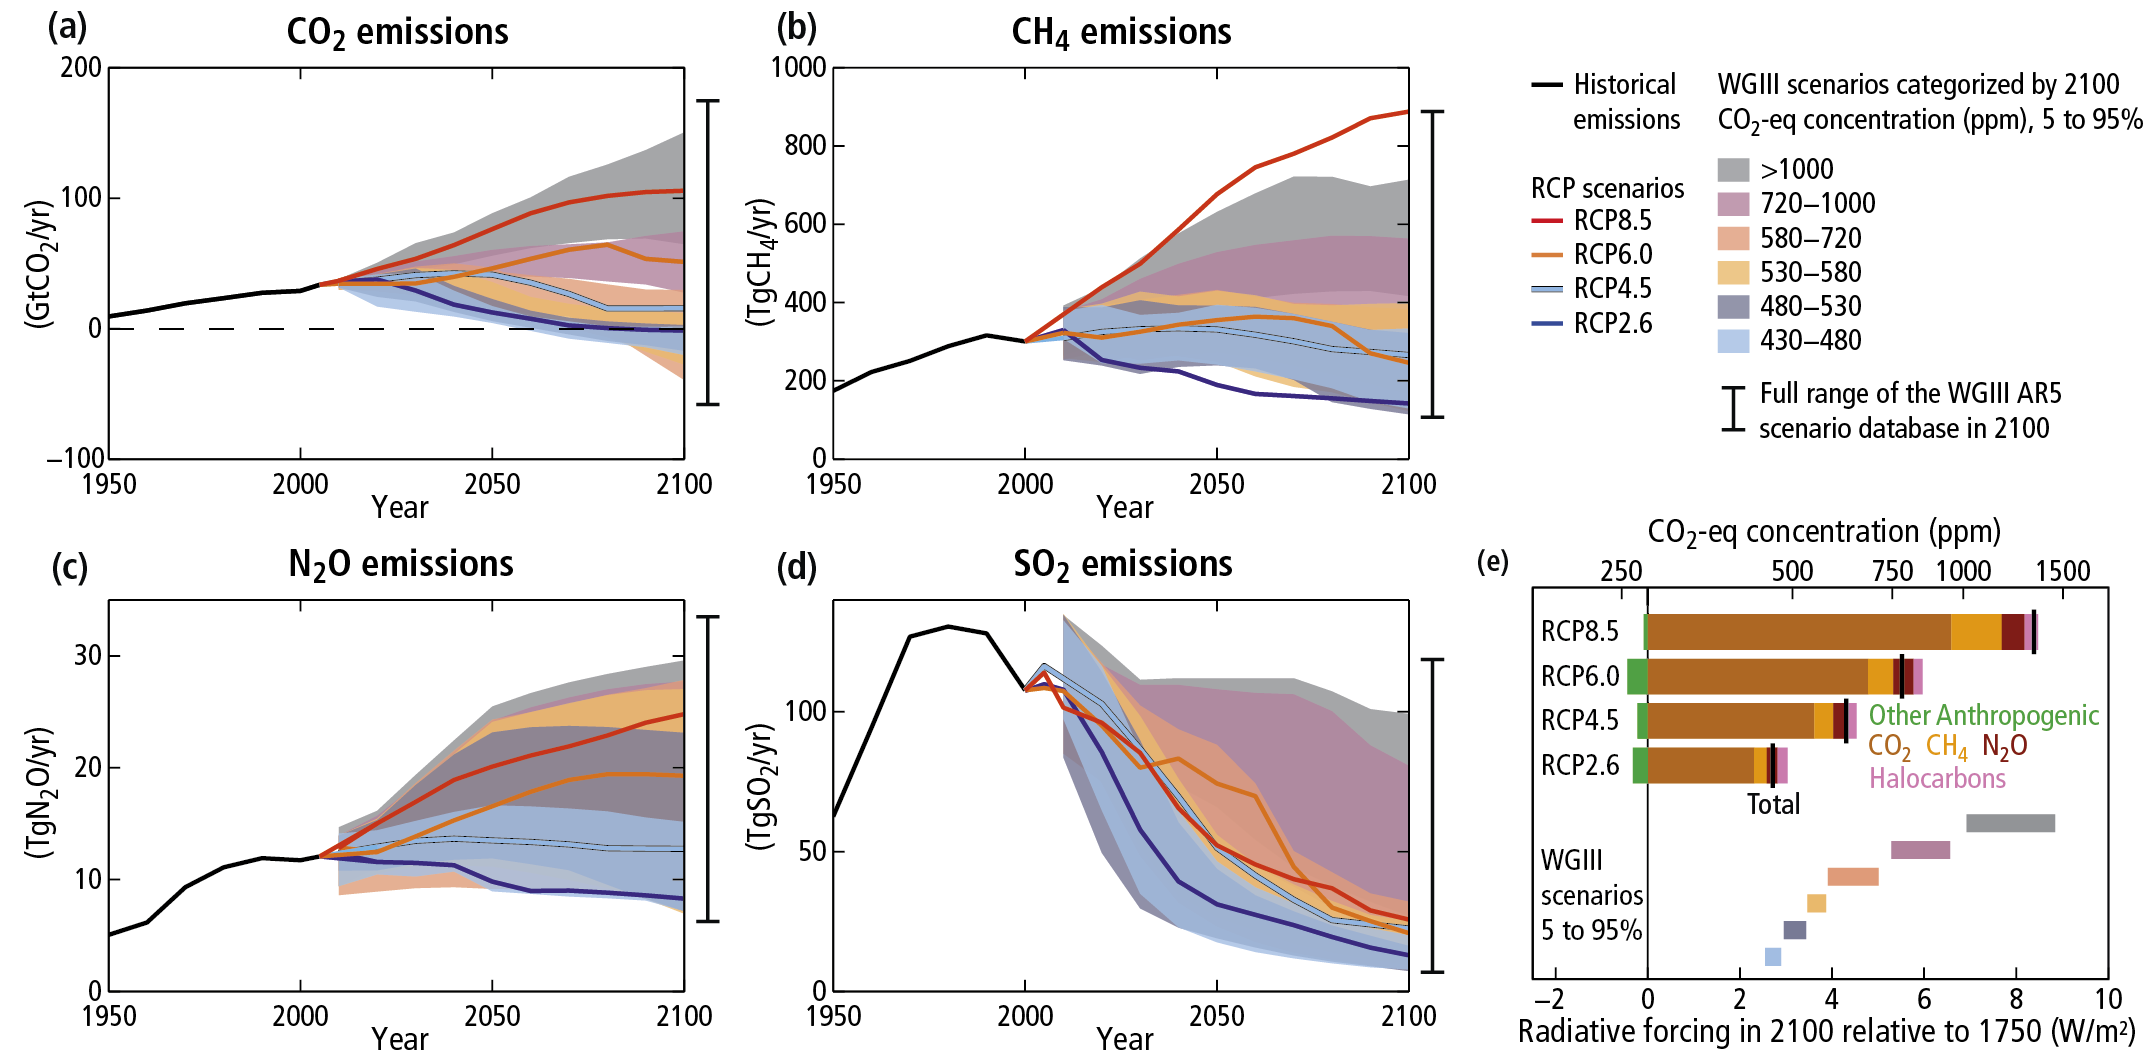
\includegraphics[width=1.2\linewidth]{figs/ipcc3} \caption{Serie de emisiones)}\label{fig:unnamed-chunk-24}
\end{figure}

\begin{figure}
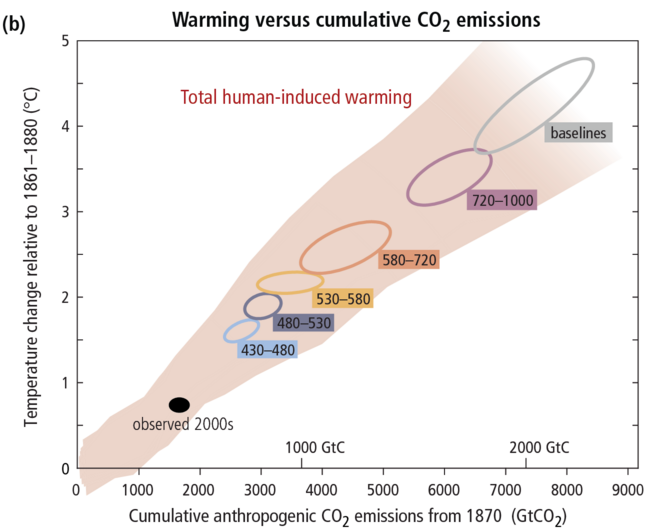
\includegraphics[width=1.5\linewidth]{figs/ipcc4} \caption{CO2 y temperatura (http://www.ipcc.ch/report/graphics/))}\label{fig:unnamed-chunk-25}
\end{figure}

\hypertarget{calidad-y-criterio}{%
\subsection{Calidad y criterio}\label{calidad-y-criterio}}

Un inventario de emisiones debe considerar la aseguracion de la calidad. En este sentido, los cientificos buscan errores, puntos debiles. Los tomadores de decisiones (UNFCC-IPCC) buscan consenso.
Por lo tanto, la calidad para los inventarios cientificos consiste en que las estimaciones tienen que ser confirmadas, calibradas y validadas. Y en el plano politico, un inventario de calidad genera in acuerdo y protocolo que todos deben atacar (VEA CLRTAP)

\hypertarget{dimensiones}{%
\subsection{Dimensiones}\label{dimensiones}}

Como \textbf{cientificos} necesitamos responder las siguentes preguntas:

\begin{itemize}
\tightlist
\item
  Que: Que contaminante (especifico) es emitido.
\item
  Como: Cual es el proceso.
\item
  Cuando: Caracterizacion temporal.
\item
  Onde: Caracterizacion temporal.
\end{itemize}

** Mapas interactivos de Inventario de emisiones vehiculares de Sao Paulo (Ibarra 2017)**

\begin{itemize}
\tightlist
\item
  \href{http://jornal.usp.br/wp-content/uploads/gPM.html}{PM2.5}
\item
  \href{http://jornal.usp.br/wp-content/uploads/gNOx.html}{NOx}
\item
  \href{http://jornal.usp.br/wp-content/uploads/gCO.html}{CO}
\item
  \href{http://jornal.usp.br/wp-content/uploads/gHC.html}{HC}
\end{itemize}

\hypertarget{categorias-llave}{%
\subsection{Categorias llave}\label{categorias-llave}}

En los inventarios de emisiones muchas veces pocas categorias emiten la mayor cantidad de contaminantes. Estas son las \textbf{categorias llave} y es en ellas donde debemos invertir la mayor cantidad de esfuerzo y recurso economico.

\hypertarget{bottom-up-y-top-down}{%
\subsection{Bottom-up y top-down}\label{bottom-up-y-top-down}}

En las guias de emisiones europeas, \citeyearpar{NtziachristosSamaras2016} muestra la definicion de los enfoques bottom-up y top-down.

\begin{figure}
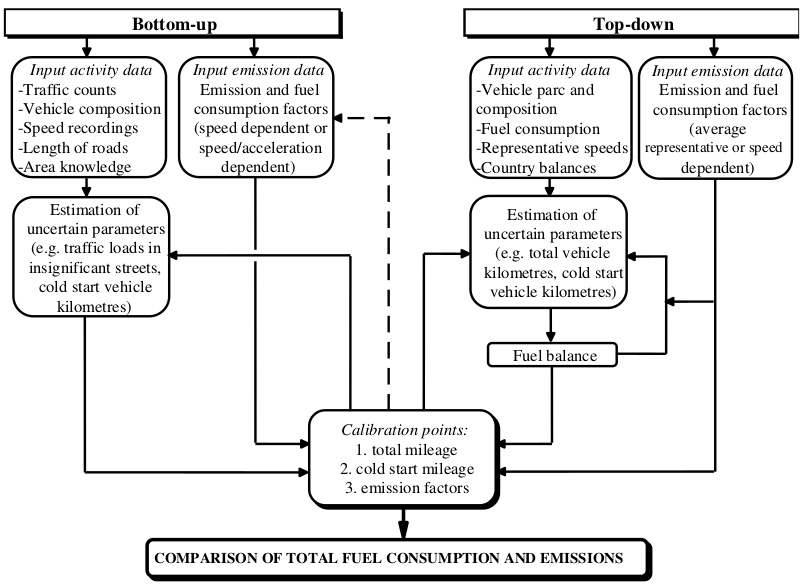
\includegraphics[width=1.2\linewidth]{figs/bt} \caption{Bottom up y top-down}\label{fig:unnamed-chunk-26}
\end{figure}

\hypertarget{ejemplo-de-factores-de-emision-real-time-gps}{%
\subsection{Ejemplo de factores de emision (real-time GPS)}\label{ejemplo-de-factores-de-emision-real-time-gps}}

\begin{figure}
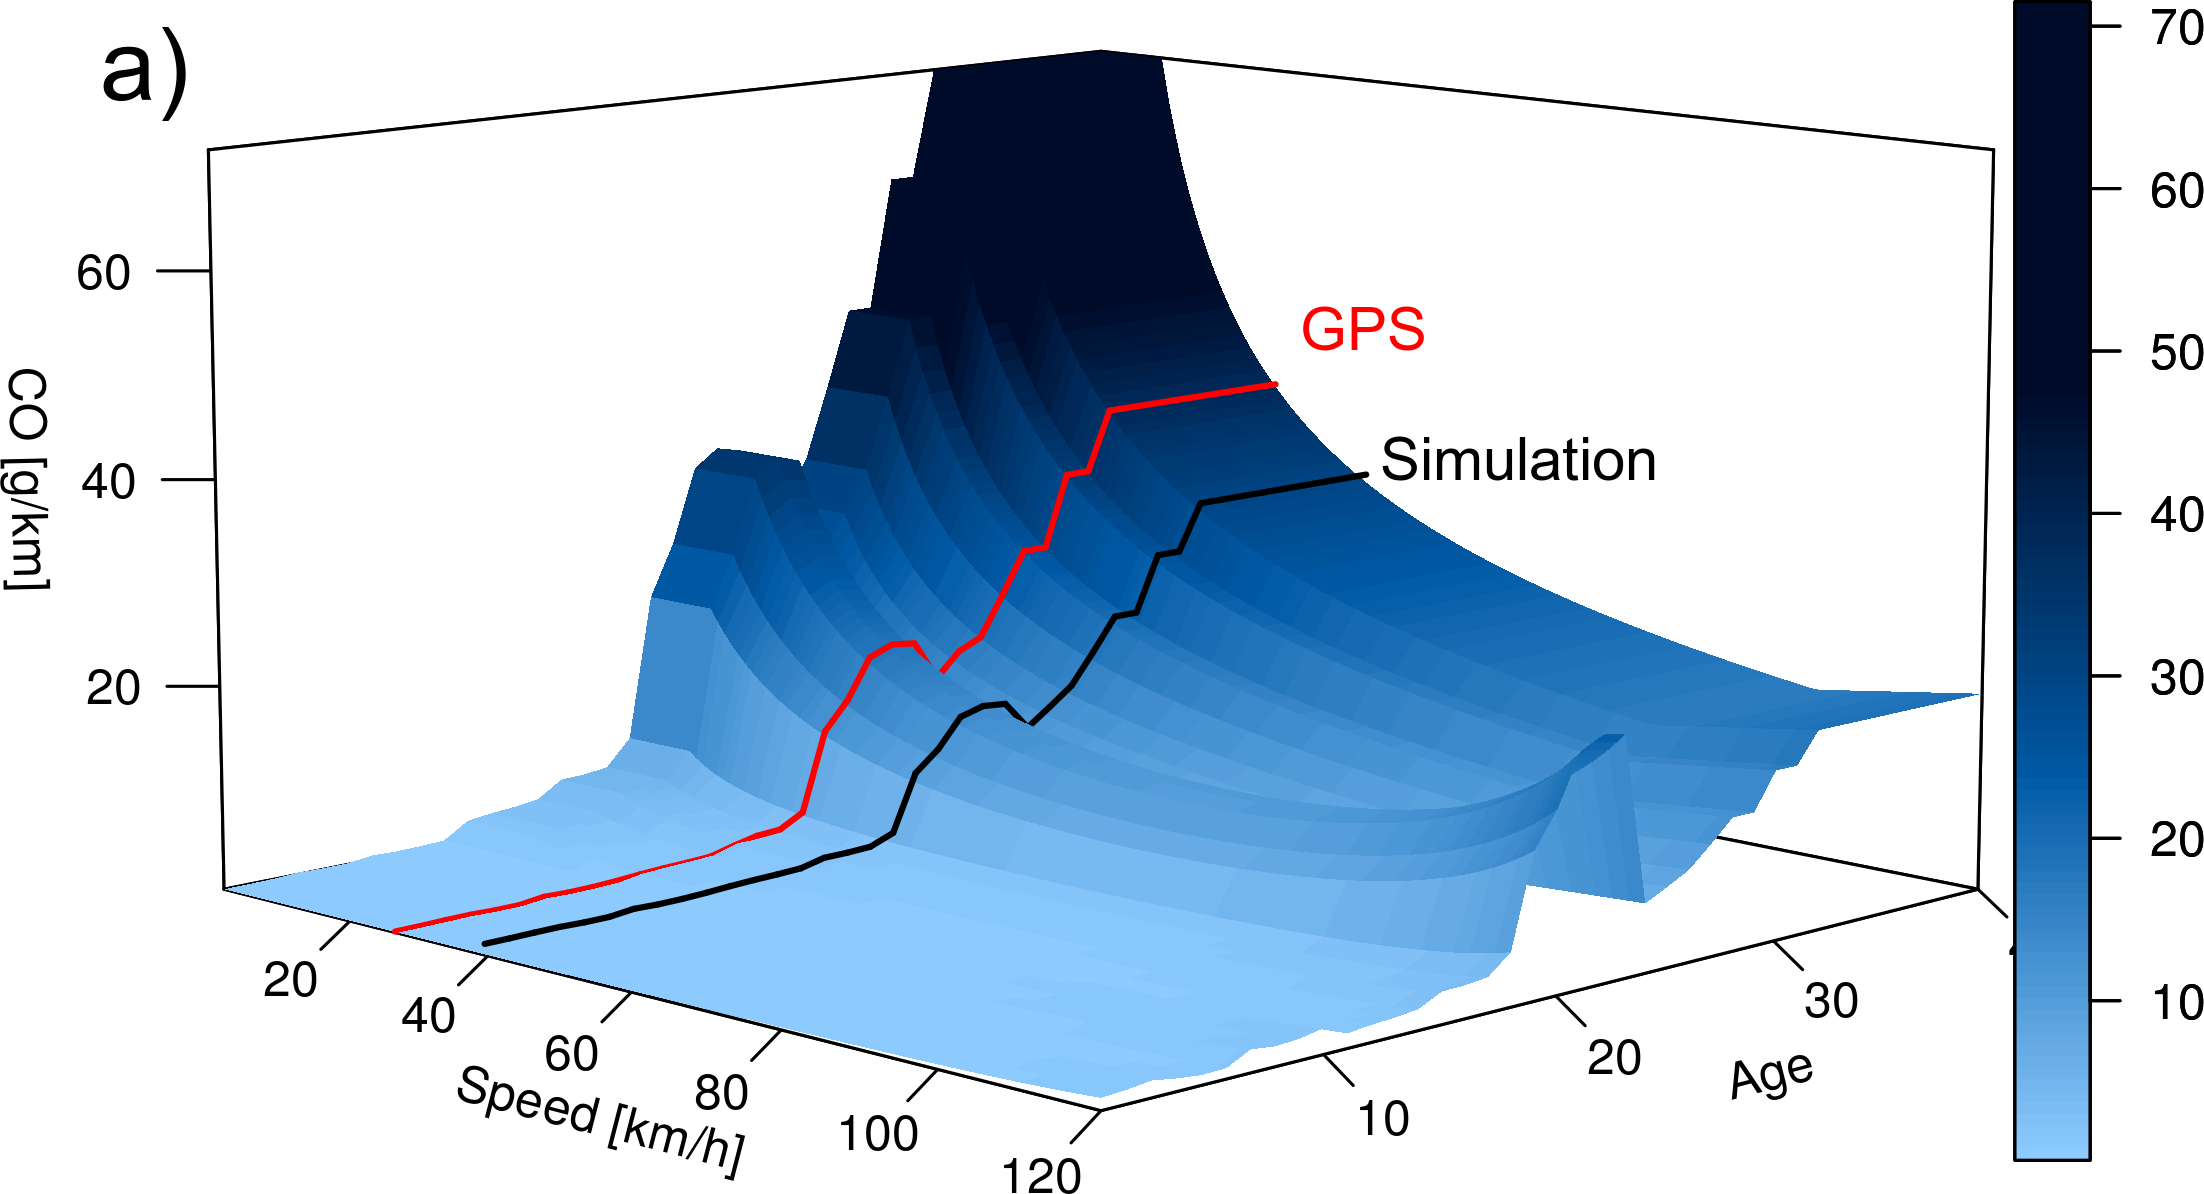
\includegraphics[width=30.61in]{figs/fig4_LDV_CO} \caption{(Ibarra-Espinosa et al., 2019 under-review)}\label{fig:unnamed-chunk-27}
\end{figure}

\hypertarget{nuevos-modelos-de-emisiones-vein}{%
\section{Nuevos modelos de emisiones: VEIN}\label{nuevos-modelos-de-emisiones-vein}}

En el ultimo par de años se han publicado nuevos modelos para el calculo de emisiones, como el Vehicular Emissions Inventory model \citep{gmd} que consiste en una libreria en R (\url{https://atmoschem.github.io/vein/}).

\begin{figure}
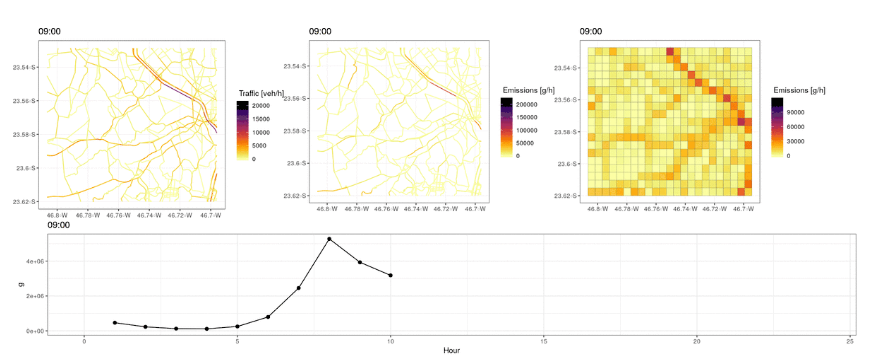
\includegraphics[width=1.3\linewidth]{figs/vein1} \caption{(Ibarra-Espinosa et al., 2018, https://atmoschem.github.io/vein/)}\label{fig:unnamed-chunk-28}
\end{figure}

\begin{figure}
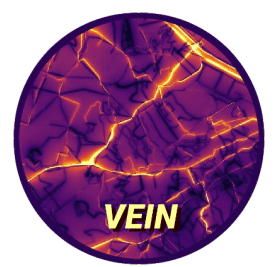
\includegraphics[width=1.3\linewidth]{figs/vein2} \caption{(Ibarra-Espinosa et al., 2018, https://atmoschem.github.io/vein/)}\label{fig:unnamed-chunk-29}
\end{figure}

\hypertarget{nuevos-datos-satelites-y-modelacion-inversa}{%
\section{Nuevos datos, satelites y modelacion inversa}\label{nuevos-datos-satelites-y-modelacion-inversa}}

La modelacion inversa esta siendo utilizada para corregir y re estimar emisiones con los nuevos datos de satelite disponibles \citep{acp-18-5483-2018}:

\begin{figure}
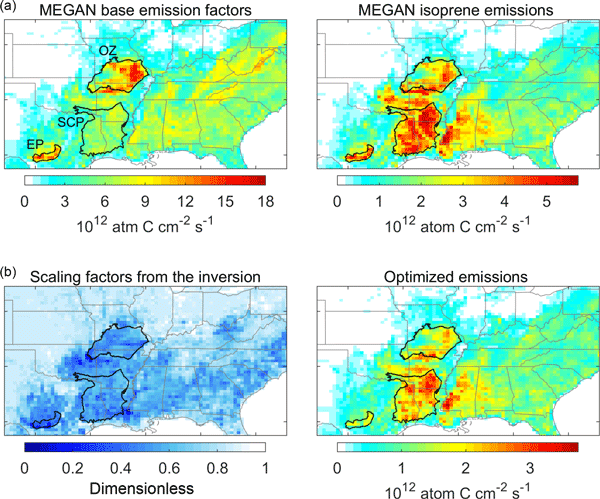
\includegraphics[width=1.3\linewidth]{figs/acp} \caption{(Kaiser et al., 2018)}\label{fig:unnamed-chunk-30}
\end{figure}

Columna total de NO2 en europa con Sentinel 5P libreria stars \citep{stars}

\begin{figure}
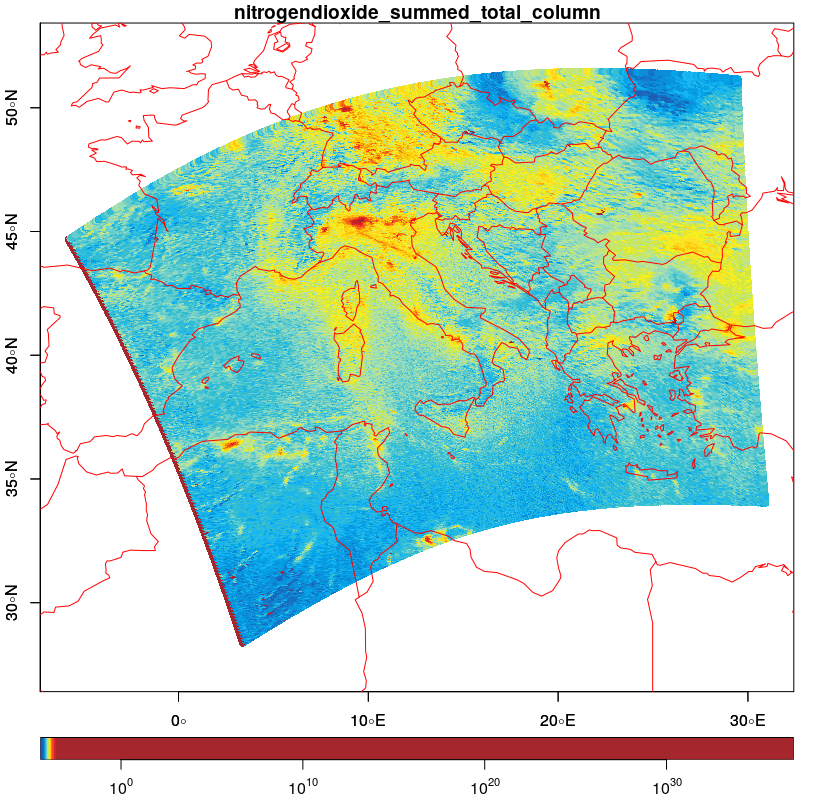
\includegraphics[width=1.5\linewidth]{figs/sentinel} \caption{STARS! Sentinel 5P}\label{fig:unnamed-chunk-31}
\end{figure}

\hypertarget{taller-vectores-aplicacion-de-software-de-informacion-geografica-y-modelado-no-terminado}{%
\chapter{Taller VECTORES: Aplicación de software de información geográfica y modelado (no terminado)}\label{taller-vectores-aplicacion-de-software-de-informacion-geografica-y-modelado-no-terminado}}

\textbf{Nota: Existen diferentes recursos para aprender R, sf, stars y raster. Use Google, Baidu o duckduckgo}

\begin{itemize}
\tightlist
\item
  www.github.com/r-spatial/sf
\item
  www.github.com/r-spatial/stars
\item
  www.github.com/rspatial/raster
\item
  \url{https://bookdown.org/}
\item
  \url{https://geocompr.robinlovelace.net/}
\item
  \url{https://www.datascienceatthecommandline.com/}
\item
  \url{https://bookdown.org/rdpeng/rprogdatascience/}
\end{itemize}

\hypertarget{instalacion}{%
\section{Instalacion}\label{instalacion}}

Por favor instale las siguientes librerias en R, copie y peque (cole) en R:

\begin{Shaded}
\begin{Highlighting}[]
\KeywordTok{install.packages}\NormalTok{(}
  \KeywordTok{c}\NormalTok{(}\StringTok{"sf"}\NormalTok{, }\StringTok{"stars"}\NormalTok{, }\StringTok{"cptcity"}\NormalTok{, }\StringTok{"ggplot2"}\NormalTok{, }\StringTok{"raster"}\NormalTok{, }\StringTok{"ncdf4"}\NormalTok{, }
    \StringTok{"RNetCDF"}\NormalTok{, }\StringTok{"maps"}\NormalTok{, }\StringTok{"data.table"}\NormalTok{, }\StringTok{"readxl"}\NormalTok{)}
\NormalTok{)}
\end{Highlighting}
\end{Shaded}

Para correr el ejemplo de stars con Sentinel 5P instale la sigueinte libreria (1 Gb)

\begin{Shaded}
\begin{Highlighting}[]
\KeywordTok{install.packages}\NormalTok{(}
  \KeywordTok{c}\NormalTok{(}\StringTok{"starsdata"}\NormalTok{)}
\NormalTok{)}
\end{Highlighting}
\end{Shaded}

Para realmente comenzar es necesario mencionar que R es un lenguaje de programacion estadistico libre (gratis y abierto) orientado a objeto escrito en C, con bindings directos para C++, C y Fortran.

\hypertarget{r-desde-excel-libreoffice-archivos-de-text-etc.}{%
\section{R desde Excel, libreoffice, archivos de text, etc.}\label{r-desde-excel-libreoffice-archivos-de-text-etc.}}

A veces debemos o obtenemos datos en hojas de calculo (Libreoffice Calc o Microsoft Office Excel). Cuando este archivo es pequeño no hay problema, pero la realidad es que cada vez es mas frecuente contar con grandes bases de datos y trabajar con un programa de interface grafica se hace dificil. Una de las razones es que la interfaz grafica consume muchos recursos computacionales, que podrian ser usados para el procesamiento de informacion. Por lo tanto

\textbf{do (5 min)}

\begin{itemize}
\tightlist
\item
  Abra el archivo dados/o3.csv con Excel
\item
  Vea rapidamente los datos
\item
  Cierre y abrael archivo con un editor de texto (bloc de notas)
\item
  Cual es la separacion de las columnas?
\item
  Bajando datos de ozono: \url{https://sinca.mma.gob.cl/index.php/estacion/index/key/D13}
\end{itemize}

\hypertarget{usando-base}{%
\subsection{Usando base}\label{usando-base}}

\begin{Shaded}
\begin{Highlighting}[]
\NormalTok{df <-}\StringTok{ }\KeywordTok{read.csv}\NormalTok{(}\StringTok{"dados/o3.csv"}\NormalTok{, }\DataTypeTok{h =}\NormalTok{ T, }\DataTypeTok{sep =} \StringTok{";"}\NormalTok{)}
\KeywordTok{head}\NormalTok{(df)}
\KeywordTok{names}\NormalTok{(df) <-}\StringTok{ }\KeywordTok{c}\NormalTok{(}\StringTok{"YYMMDD"}\NormalTok{, }\StringTok{"HHMM"}\NormalTok{, }\StringTok{"o3_ppb"}\NormalTok{, }\StringTok{"novalido"}\NormalTok{)}
\end{Highlighting}
\end{Shaded}

\hypertarget{usando-data.table-mi-favorito-junto-con-sf}{%
\subsection{Usando data.table (mi favorito junto con sf)}\label{usando-data.table-mi-favorito-junto-con-sf}}

data.table es mas rapido que python, julia y spark

\textbf{\url{https://h2oai.github.io/db-benchmark/}}

\begin{Shaded}
\begin{Highlighting}[]
\KeywordTok{library}\NormalTok{(data.table)}
\NormalTok{df <-}\StringTok{ }\KeywordTok{fread}\NormalTok{(}\StringTok{"data/china_cities_20190413.csv"}\NormalTok{)}
\KeywordTok{head}\NormalTok{(df)}
\end{Highlighting}
\end{Shaded}

\hypertarget{usndo-readxl}{%
\subsection{Usndo readxl}\label{usndo-readxl}}

\begin{Shaded}
\begin{Highlighting}[]
\KeywordTok{library}\NormalTok{(readxl)}
\NormalTok{df <-}\StringTok{ }\KeywordTok{read_xlsx}\NormalTok{(}\StringTok{"data/china_cities_20190413.xlsx"}\NormalTok{)}
\KeywordTok{head}\NormalTok{(df)}
\end{Highlighting}
\end{Shaded}

\hypertarget{representacion-de-objetos-espaciales}{%
\section{Representacion de objetos espaciales}\label{representacion-de-objetos-espaciales}}

Nuevo estandard ISO (puntos, areas, lineas, volume, etc)

\hypertarget{taller-raster-y-cubos-de-datos-vectoriales-aplicacion-de-software-de-informacion-geografica-y-modelado-no-terminado}{%
\chapter{Taller RASTER Y CUBOS DE DATOS VECTORIALES: Aplicación de software de información geográfica y modelado (no terminado)}\label{taller-raster-y-cubos-de-datos-vectoriales-aplicacion-de-software-de-informacion-geografica-y-modelado-no-terminado}}

Amanda Rehbein

Raster son informacion espaciales en una grilla espacial. Por ejemplo, vea las siguientes figuras:

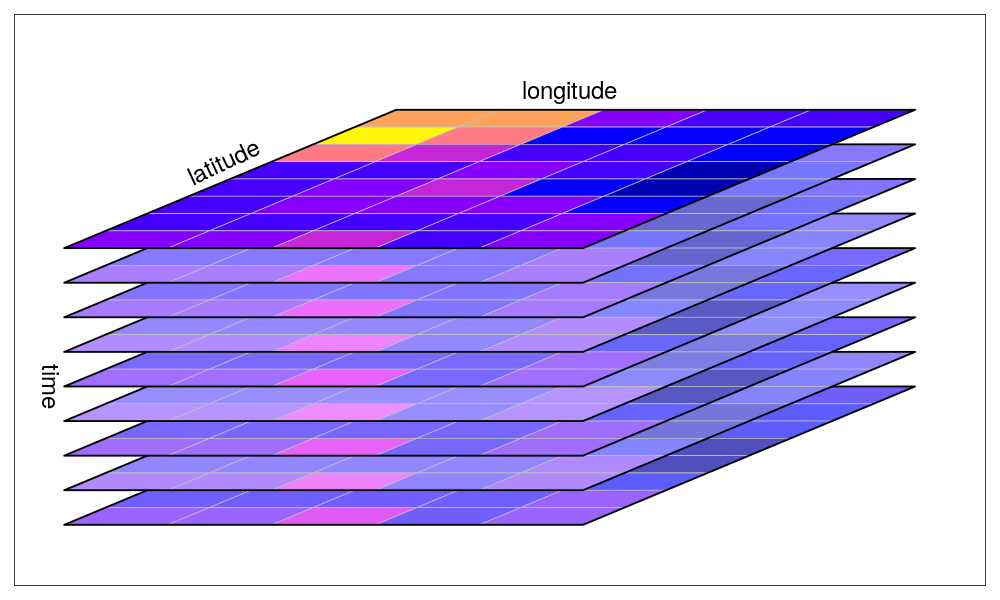
\includegraphics{figs/cube1.png}

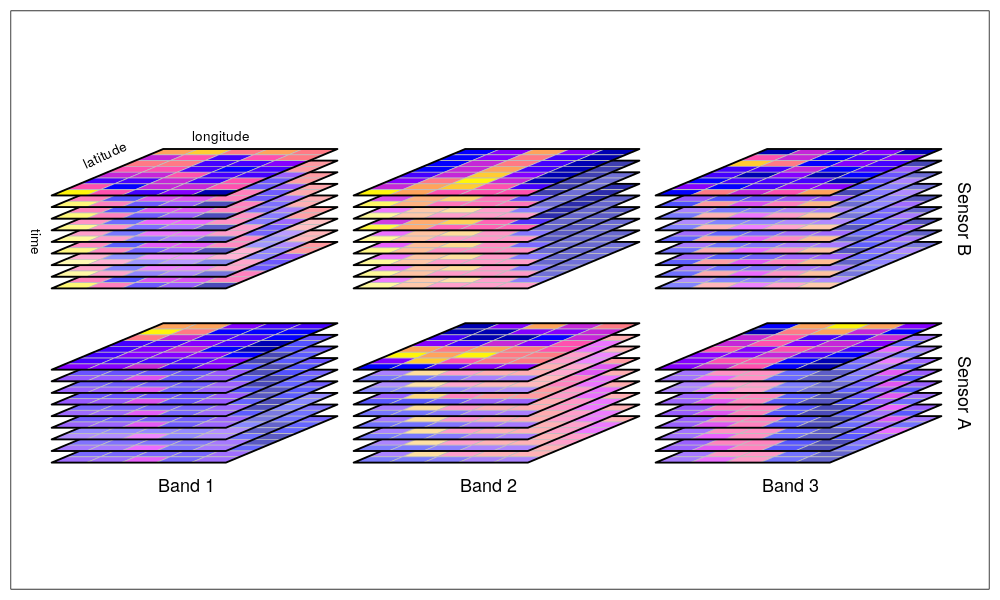
\includegraphics{figs/cube2.png}

Ejemplos con R

\hypertarget{estudios-de-series-de-tiempo-para-asociar-salud-y-variables-ambientales}{%
\chapter{Estudios de series de tiempo para asociar salud y variables ambientales}\label{estudios-de-series-de-tiempo-para-asociar-salud-y-variables-ambientales}}

Uno de los metodos mas validados y establecidos para identificar asociaciones entre mortalidad, morbilidad, y otros parametros con variables ambientales son las series de tiempo.

Algunos de los autores clasicos sobre este tipo de estudios estan:

\begin{itemize}
\tightlist
\item
  Francesca Dominici {[}link google scholar{]}
\item
  Luis Cifuentes {[}link google scholar{]}
\item
  Petros Koutrakis {[}link google scholar{]}
\item
  Paulo Saldiva {[}link google scholar{]}
\item
  Michelle Bell {[}link google scholar{]}
\item
  Antonela Zanometti {[}link google scholar{]}
\end{itemize}

Francesca Dominici ha publicado diferentes estudios y actualizado la metodologia de estudios de series de tiempo considerando la distribucion estadistica, control de los factores de confusion y modelos generales aditivos.

\hypertarget{distribucion}{%
\section{Distribucion}\label{distribucion}}

Los estudios de series de tiempo consideran en general variables diarias. En este sentido, las variables de salud son conteos diarios con una distribucion apropiada, generalmente Poisson o Binomail Negativa, por ejemplo. Estas son diferentes de la distribucion normal.

Densidad de la distribucion de Poisson:

\begin{equation}
p(x) = \lambda^x exp(-\lambda)/x!
\label{eq:12}
\end{equation}

Densidad de la distribucion de Normal:

\begin{equation}
f(x) = 1/( (2 \pi) \sigma) e^-((x - \mu)^2/(2 \sigma^2)^0.5 )
\label{eq:13}
\end{equation}

Vamos a ver un ejemplo:

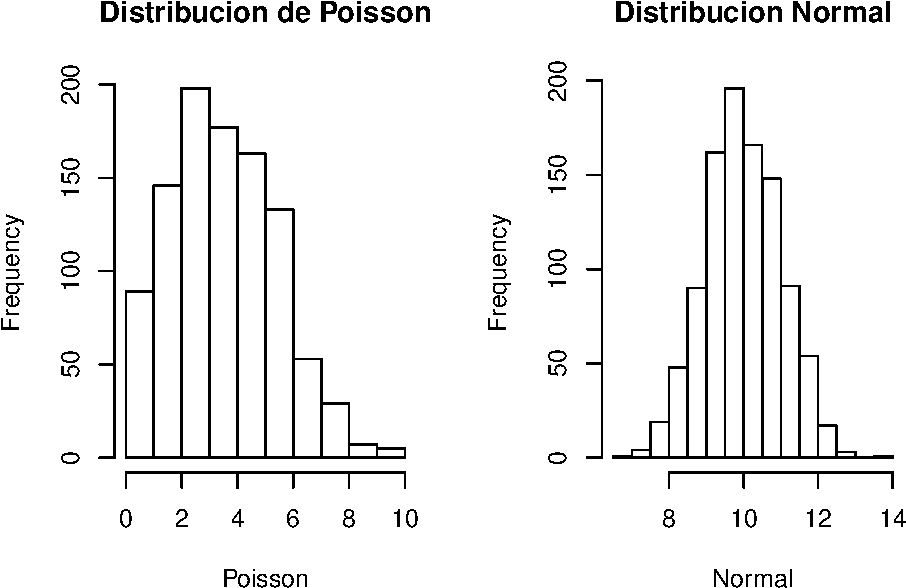
\includegraphics[height=1.5\textheight]{bookdown-demo_files/figure-latex/unnamed-chunk-38-1}

\hypertarget{efecto-de-la-contaminacion}{%
\section{Efecto de la contaminacion}\label{efecto-de-la-contaminacion}}

Dominici presento el modelo semi-parametrico usando modelos generales aditivos \citep{gam} para el estudio de series de tiempo. Este modelo consiste en:

\begin{equation}
log(m) = \beta_0 + \beta_1 \cdot X_i + s(meteo) + s(time) + s(season) + ...
\label{eq:13}
\end{equation}

Donde m es la variable dependiente sobre salud, \(\beta\) son los coeficientes, \(X_i\) son los contaminantes, \(s\) es una funcion spline

Luego, la asociacion resultante es el riesgo relativo \citep{rosana}:

\begin{equation}
RR = exp(\beta_i \cdot \delta X_i)
\label{eq:13}
\end{equation}

Que indica el riesgo relativo dada un cambio en la variable, por ejemplo, si se incrementan las concentraciones de PM10 en 50 ug/m3, el riesgo de mortalidad respiratoria aumenta 7\%. Aplicando este porcentaje sobre la poblacion es posible calcular la mortalidad anual asociada a la contaminacion. Vamos a ver valores reales para Argentina y Chile \citep{rosana}.

\begin{figure}
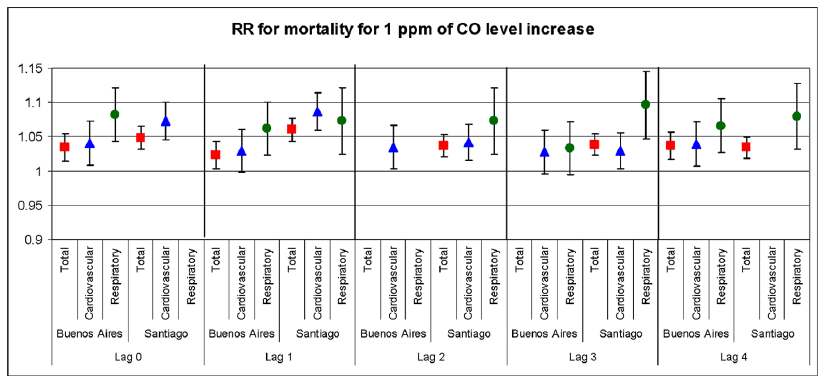
\includegraphics[width=11.44in,height=1.8\textheight]{figs/rosana1} \caption{Riesgo relativo en mortalidad por incremento de 1 ppm de CO (Abrutzky et al., 2013)}\label{fig:unnamed-chunk-39}
\end{figure}

\hypertarget{efecto-de-la-temperatura}{%
\section{Efecto de la temperatura}\label{efecto-de-la-temperatura}}

Puede se utilizada la misma metodologia pero considerando variables meteorologicas en este caso. Un trabajo muy interesante recientemente publicado por el grupo de Paulo Saliva es el efecto de la temperatura en diferentes ciudades del mundo \citep{GASPARRINI2015369}.

\begin{figure}
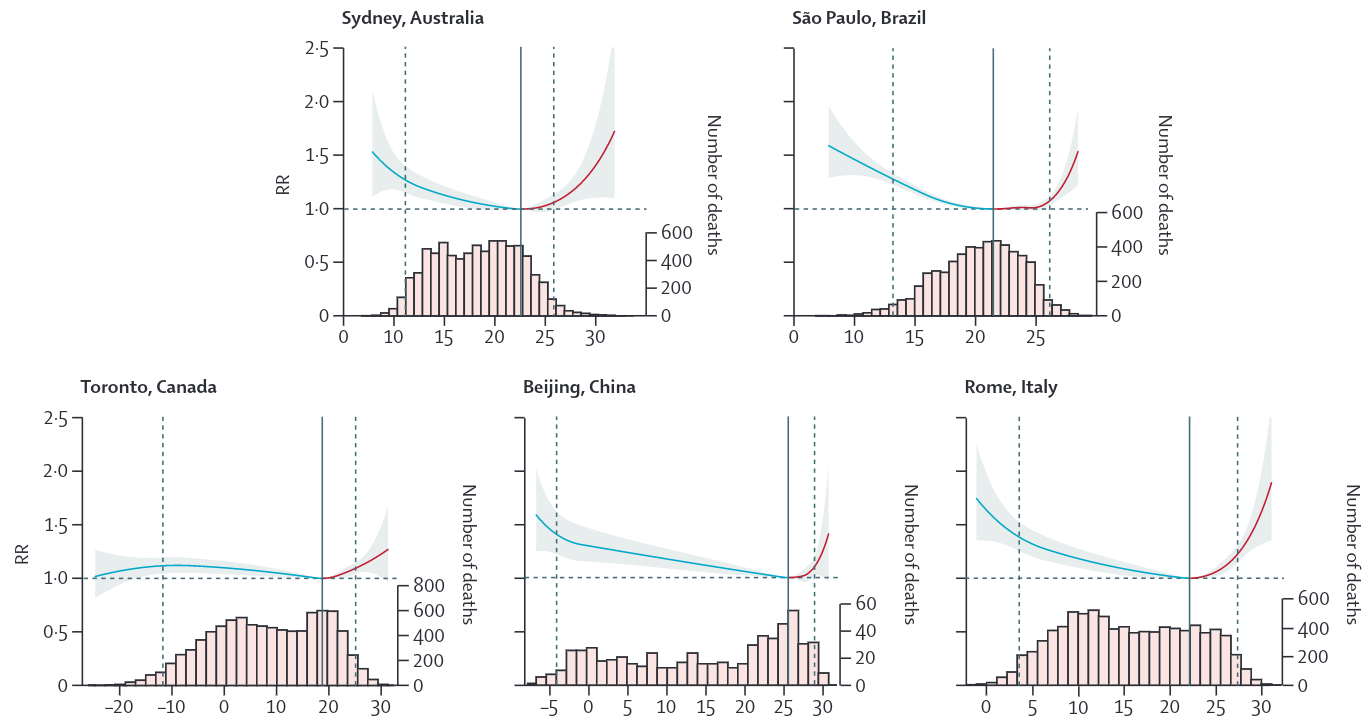
\includegraphics[width=18.97in,height=1.8\textheight]{figs/temp1} \caption{Riesgo relativo en mortalidad por incremento de 1 ppm de CO (Abrutzky et al., 2013)}\label{fig:unnamed-chunk-40}
\end{figure}

\bibliography{book.bib,packages.bib}


\end{document}
